% Options for packages loaded elsewhere
\PassOptionsToPackage{unicode}{hyperref}
\PassOptionsToPackage{hyphens}{url}
\documentclass[
  preprint]{elsarticle}
\usepackage{xcolor}
\usepackage{amsmath,amssymb}
\setcounter{secnumdepth}{5}
\usepackage{iftex}
\ifPDFTeX
  \usepackage[T1]{fontenc}
  \usepackage[utf8]{inputenc}
  \usepackage{textcomp} % provide euro and other symbols
\else % if luatex or xetex
  \usepackage{fontspec}
  \usepackage{xeCJK}
  \setmainfont{Times New Roman}
  \setCJKmainfont{Microsoft YaHei}
  \setCJKsansfont{Microsoft YaHei}
  \setCJKmonofont{Microsoft YaHei}
\fi
\ifPDFTeX
  \usepackage{lmodern}
\fi
% Use upquote if available, for straight quotes in verbatim environments
\IfFileExists{upquote.sty}{\usepackage{upquote}}{}
\IfFileExists{microtype.sty}{% use microtype if available
  \usepackage[]{microtype}
  \UseMicrotypeSet[protrusion]{basicmath} % disable protrusion for tt fonts
}{}
\makeatletter
\@ifundefined{KOMAClassName}{% if non-KOMA class
  \IfFileExists{parskip.sty}{%
    \usepackage{parskip}
  }{% else
    \setlength{\parindent}{0pt}
    \setlength{\parskip}{6pt plus 2pt minus 1pt}}
}{% if KOMA class
  \KOMAoptions{parskip=half}}
\makeatother
\usepackage{longtable,booktabs,array}
\newcounter{none} % for unnumbered tables
\usepackage{calc} % for calculating minipage widths
% Correct order of tables after \paragraph or \subparagraph
\usepackage{etoolbox}
\makeatletter
\patchcmd\longtable{\par}{\if@noskipsec\mbox{}\fi\par}{}{}
\makeatother
% Allow footnotes in longtable head/foot
\IfFileExists{footnotehyper.sty}{\usepackage{footnotehyper}}{\usepackage{footnote}}
\makesavenoteenv{longtable}
\setlength{\LTleft}{\fill}
\setlength{\LTright}{\fill}
\AtBeginEnvironment{longtable}{%
  \scriptsize
  \setlength{\tabcolsep}{2pt}%
  \renewcommand{\arraystretch}{1.16}%
  \sloppy
}
\usepackage{graphicx}
\makeatletter
\newsavebox\pandoc@box
\newcommand*\pandocbounded[1]{% scales image to fit in text height/width
  \sbox\pandoc@box{#1}%
  \Gscale@div\@tempa{\textheight}{\dimexpr\ht\pandoc@box+\dp\pandoc@box\relax}%
  \Gscale@div\@tempb{\linewidth}{\wd\pandoc@box}%
  \ifdim\@tempb\p@<\@tempa\p@\let\@tempa\@tempb\fi% select the smaller of both
  \ifdim\@tempa\p@<\p@\scalebox{\@tempa}{\usebox\pandoc@box}%
  \else\usebox{\pandoc@box}%
  \fi%
}
% Set default figure placement to htbp
\def\fps@figure{htbp}
\makeatother
\setlength{\emergencystretch}{3em} % prevent overfull lines
\providecommand{\tightlist}{%
  \setlength{\itemsep}{0pt}\setlength{\parskip}{0pt}}
\usepackage{bookmark}
\IfFileExists{xurl.sty}{\usepackage{xurl}}{} % add URL line breaks if available
\urlstyle{same}
% fallback for those not using the hyperref driver hyperxmp:
\makeatletter
\@ifundefined{xmpquote}{\newcommand{\xmpquote}[1]{#1}}{}
\makeatother
\hypersetup{
  pdftitle={A Low-Latency and Energy-Efficient FPGA Architecture for Partially Coherent Lithographic Aerial Image Computation},
  hidelinks,
  pdfcreator={LaTeX via pandoc}}

\title{A Low-Latency and Energy-Efficient FPGA Architecture for Partially Coherent Lithographic Aerial Image Computation}
\author{}
\date{}

\begin{document}
\begin{frontmatter}
\maketitle

\begin{highlights}
\item
  A CPU-FPGA collaborative acceleration framework is proposed for online
  TCC-SOCS aerial image reconstruction in computational lithography. It
  decouples offline preprocessing performed when optical parameters
  change from online reconstruction repeatedly invoked for mask windows,
  reducing online latency and improving energy efficiency while
  preserving model accuracy and configurability.
\item
  The \(17 \times 17\) SOCS eigenkernels are embedded into a fixed
  \(128 \times 128\) FFT grid, and an area-optimized two-dimensional
  complex IFFT datapath is designed so that the same online
  reconstruction pipeline can accommodate different effective kernel
  sizes.
\item
  Block-floating-point dynamic-range compensation, multiple independent
  AXI-MM interfaces, and BRAM buffering are combined to reduce resource
  consumption and memory-access contention during two-dimensional IFFT
  and multi-kernel accumulation.
\item
  Host-FPGA PCIe on-board validation is completed using Xilinx XDMA. On
  the xcku5p, the 10-kernel online reconstruction kernel achieves a
  latency of 10.57 ms and a \(3.37\times\) speedup over the C++ SOCS
  baseline.
\end{highlights}

\begin{abstract}

Online aerial image reconstruction based on the transmission cross
coefficient (TCC) and the sum of coherent systems (SOCS) is a frequently
invoked computational bottleneck in computational lithography workflows
such as optical proximity correction, source-mask optimization, and
inverse lithography technology, where conventional CPU platforms
struggle to balance latency and energy efficiency under power
constraints. To address this problem, this paper proposes a decoupled
CPU-FPGA collaborative acceleration architecture: the CPU performs
offline TCC construction and SOCS eigenkernel extraction, while the FPGA
executes online frequency-domain embedding, two-dimensional IFFT, and
weighted accumulation through an area-efficient datapath combining a
fixed FFT grid, block-floating-point compensation, multiple AXI-MM
interfaces, and BRAM buffering. Compared with an optimized C++ SOCS
baseline implementing the same online reconstruction operator, the
proposed FPGA kernel achieves a \(3.37\times\) speedup and, based on
current power estimates, an approximately \(67.4\times\) improvement in
kernel-only energy efficiency, demonstrating its effectiveness for
low-power online reconstruction in computational lithography.

\end{abstract}

\begin{keyword}
computational lithography \sep TCC-SOCS \sep CPU-FPGA collaboration \sep FPGA acceleration \sep energy-efficient computing
\end{keyword}
\end{frontmatter}

\section{1. Introduction}\label{introduction}

Computational lithography has become a key technology connecting optical
imaging, process-window analysis, and layout optimization in advanced
semiconductor manufacturing. As process nodes continue to shrink,
improving resolution solely through projection optics has become
increasingly difficult. Optical proximity correction (OPC), source-mask
optimization (SMO), and inverse lithography technology (ILT) are
therefore widely used to compensate for proximity effects, optimize
illumination and mask geometries, and enlarge manufacturable process
windows {[}1{]}-{[}11{]}. These techniques generally operate through
model feedback or inverse-problem optimization and require frequent
aerial image computation over numerous layout windows, process
conditions, and optimization iterations {[}2{]}, {[}3{]}, {[}5{]},
{[}8{]}. As process windows narrow, mask complexity increases, and
optimization variables evolve from edge displacements to pixelated or
curvilinear patterns, the latency, throughput, and energy consumption of
aerial image computation have become major bottlenecks in the practical
deployment of computational lithography.

Partially coherent lithographic imaging is commonly formulated using
Hopkins theory. Its transmission cross coefficient (TCC) represents the
illumination source, projection pupil, aberrations, thin-film effects,
and mask spectrum/diffracted-order map within a unified frequency-domain
operator {[}12{]}-{[}18{]}. When the optical parameters remain fixed,
the TCC can be precomputed offline and reused across different mask
patterns. Direct TCC imaging, however, involves dense coupling between
frequency pairs and consequently incurs substantial computational and
storage costs. The sum of coherent systems (SOCS) method applies
eigendecomposition or low-rank approximation to the TCC, converting
partially coherent imaging into a weighted sum of coherent eigenkernels.
It thereby reduces online computational complexity while retaining the
physical interpretability of the imaging model {[}12{]}, {[}13{]},
{[}16{]}, {[}19{]}. TCC-SOCS has consequently become an important
approach for balancing accuracy and efficiency in aerial image
computation.

Although SOCS transforms the dense frequency coupling of direct TCC
imaging into a weighted sum of a finite number of coherent systems,
online reconstruction remains a frequently executed computational
hotspot after the offline decomposition. For each SOCS eigenkernel,
online reconstruction requires multiplication of the mask spectrum by
the eigenkernel, a 2D IFFT, magnitude-squared evaluation, eigenvalue
weighting, and multi-kernel intensity accumulation. These operations are
repeated in proportion to the number of eigenkernels, mask windows, and
OPC/SMO/ILT iterations {[}19{]}-{[}23{]}. In batch window evaluation,
process-window scanning, or iterative mask optimization, the SOCS
eigenkernels, weights, and control configuration can be reused across a
large number of windows under the same optical condition. Reductions in
the latency and energy consumption of a single online reconstruction
therefore accumulate into substantial improvements in batch throughput.
The engineering value of a low-power, deterministic online operator
extends beyond single-frame acceleration to pipelined processing of
mask-window batches, edge-oriented critical-dimension verification, and
system-level energy budgeting.

Previous studies have improved the efficiency of lithography simulation
or mask optimization through numerical approximation, symmetry
exploitation, CPU/GPU acceleration, and learning-based models {[}20{]},
{[}22{]}-{[}30{]}. CPUs offer high flexibility but limited energy
efficiency for regular frequency-domain operations. GPUs provide high
throughput for large batches, but their system power consumption of
several hundred watts, host-side scheduling overhead, and
nondeterministic interrupt latency can restrict their applicability in
low-power critical-dimension verification, distributed edge-computing
nodes, and compact hardware integration. FPGAs provide a complementary
alternative to CPUs and GPUs for online TCC-SOCS reconstruction. Complex
multiplication, two-dimensional IFFT, magnitude-squared evaluation, and
accumulation all exhibit regular datapaths and explicit dependencies
suitable for deterministic pipelines. On-chip BRAM can cache
intermediate matrices to reduce round trips to DDR, while multiple
AXI-MM interfaces can mitigate memory-access contention among the mask
spectrum, SOCS eigenkernels, weights, and output buffers.

Existing studies have demonstrated the potential of FPGAs for
lithographic aerial image simulation and two-dimensional FFT
acceleration, and have identified the trade-offs among external-memory
access, row-column transposition, parallelism, and energy efficiency as
critical to FFT-based hardware accelerators {[}31{]}-{[}38{]}.
Nevertheless, prior computational lithography acceleration studies have
focused primarily on algorithmic approximation, CPU/GPU implementations,
learning-based OPC/ILT, or FPGA lithography simulation outside the
TCC-SOCS formulation. A unified treatment of a dedicated FPGA/HLS
datapath for online TCC-SOCS reconstruction, the Host-FPGA XDMA
dataflow, the physical hardware control path, and end-to-end error
validation remains lacking. In other words, existing work has not fully
established how latency, bandwidth, accuracy, resource consumption, and
system-integration overhead can be balanced simultaneously for online
TCC-SOCS reconstruction under limited FPGA resources.

This work focuses on the online reconstruction stage after offline TCC
construction and SOCS eigenkernel extraction, rather than accelerating
complete TCC generation, eigendecomposition, or an entire OPC/SMO
optimization system. For this online stage, a CPU-FPGA collaborative
architecture is proposed. The CPU performs offline TCC construction,
eigendecomposition, SOCS eigenkernel generation, and host-side Fourier
interpolation (FI). The FPGA performs online frequency-domain embedding,
\(128 \times 128\) two-dimensional IFFT, weighted accumulation,
FFTshift, and result write-back. PCIe XDMA is used to integrate
Host-FPGA data transfer, control configuration, and result read-back
across the complete platform. The principal contributions are fourfold.
First, a CPU-FPGA collaborative framework for online TCC-SOCS
reconstruction is established, explicitly decoupling offline optical
preprocessing, online FPGA reconstruction, and host-side
post-processing. Second, a pipeline is designed for frequency-domain
embedding of \(17 \times 17\) SOCS eigenkernels into a
\(128 \times 128\) FFT grid, two-dimensional IFFT, intensity
accumulation, FFTshift, and result write-back. Third, an area-optimized
two-dimensional complex IFFT processor is developed for the DUV cutoff
frequency and fixed FFT grid. It combines block-floating-point
dynamic-range compensation, conflict-free transpose storage, LUT-mapped
multiplication, BRAM buffering, and multiple independent AXI-MM
interfaces to reduce resource consumption and memory-access contention.
Finally, complete Host-FPGA validation based on PCIe XDMA is
demonstrated, covering input-data writes, AXI-Lite control
configuration, FPGA computation, read-back of the \(128 \times 128\)
result, and host-side Fourier interpolation to \(1024 \times 1024\).

The proposed architecture is evaluated under a fixed 10-kernel
configuration in terms of MATLAB model accuracy, CPU-FPGA performance
for the same operator, and estimated kernel-only energy efficiency. The
RMSE of the 10-kernel SOCS result relative to the full MATLAB TCC result
is \(5.472\times10^{-3}\). The on-board FPGA output has an RMSE of
\(2.93\times10^{-8}\) relative to the SOCS software Golden result under
the same configuration, demonstrating that the hardware implementation
error is substantially smaller than the model truncation error. At 250
MHz, the online reconstruction kernel has a latency of 10.57 ms,
achieving a \(3.37\times\) speedup and a 70.3\% latency reduction over
the C++ SOCS baseline. Based on estimated FPGA kernel and CPU power
consumptions of approximately 4 W and 80 W, respectively, the energy
consumption per image is reduced by approximately 98.5\%, corresponding
to an estimated \(67.4\times\) improvement in kernel-only energy
efficiency. The final architecture utilizes 17\% of the LUTs, 9\% of the
FFs, 2\% of the DSPs, and 42\% of the BRAM. The remainder of this paper
is organized as follows. Section 2 presents the TCC-SOCS model and
proposed architecture, Section 3 reports the experimental results, and
Section 4 concludes the paper.

\section{2. Principles and Methods}\label{principles-and-methods}

\subsection{2.1 TCC-SOCS Imaging Model and Problem
Definition}\label{tcc-socs-imaging-model-and-problem-definition}

For partially coherent lithographic imaging, the Hopkins formulation
expresses the aerial image intensity as a bilinear form of the mask
spectrum. The TCC is a frequency-domain kernel determined by the
illumination source and projection optics:

\[
\begin{aligned}
TCC(f',g';f'',g'')={}&\iint S(f_s,g_s)P(f'+f_s,g'+g_s)\\
&\quad\cdot P^*(f''+f_s,g''+g_s)\,df_s\,dg_s.
\end{aligned}
\tag{1}
\]

Here, \((f',g')\) and \((f'',g'')\) are the two sets of mask-frequency
coordinates involved in the TCC bilinear coupling, and \((f_s,g_s)\)
denotes the source-frequency coordinates. \(S(f_s,g_s)\) is the
non-negative source distribution, \(P(f,g)\) is the complex pupil
function incorporating the projection pupil and aberrations, and
\(P^*(f,g)\) denotes its complex conjugate. When the optical parameters
are fixed, the TCC can be precomputed and reused across different mask
patterns. The corresponding aerial image intensity is

\[
\begin{aligned}
I(x,y)={}&\iiiint TCC(f',g';f'',g'')M(f',g')M^*(f'',g'')\\
&\quad\cdot e^{j2\pi[(f'-f'')x+(g'-g'')y]}
\,df'\,dg'\,df''\,dg''.
\end{aligned}
\tag{2}
\]

Here, \((x,y)\) denotes the spatial coordinates in the image plane,
\(M(f,g)\) is the mask spectrum, \(M^*(f,g)\) is its complex conjugate,
and \(j=\sqrt{-1}\). Although this direct formulation provides high
accuracy, its dense coupling between frequency pairs entails a high
computational cost.

The TCC matrix is Hermitian and can generally be approximated by a
low-rank decomposition:

\[
TCC \approx \sum_{k=1}^{N_k}\sigma_k\Phi_k\Phi_k^*.
\tag{3}
\]

Here, \(\sigma_k\) is the eigenvalue weight of the \(k\)th component,
\(\Phi_k\) is the corresponding coherent eigenkernel in the frequency
domain, \(\Phi_k^*\) is its conjugate transpose, and \(N_k\) is the
number of retained SOCS eigenkernels. Substitution of this decomposition
into the Hopkins equation gives

\[
I(x,y) \approx
\sum_{k=1}^{N_k}\sigma_k
\left|\mathcal{F}^{-1}\{M(f,g)\Phi_k(f,g)\}\right|^2.
\tag{4}
\]

Here, \(\mathcal{F}^{-1}\{\cdot\}\) denotes the two-dimensional inverse
Fourier transform, and \(\Phi_k(f,g)\) is the \(k\)th SOCS eigenkernel
in the frequency domain. The online computation for each eigenkernel
therefore comprises frequency-domain multiplication, IFFT,
magnitude-squared evaluation, and weighted accumulation. The symbol
\(\sigma_k\) denotes only the eigenvalue weight of the \(k\)th
eigenkernel and is distinct from the outer coherence factor
\(\sigma_{out}\) in the optical configuration.

In a discrete implementation, the effective frequency-domain extent of
the TCC is determined by the pupil cutoff frequency:

\[
\begin{aligned}
N_x=N_y
&=\left\lfloor
\frac{L_x\cdot NA\cdot(1+\sigma_{out})}{\lambda}
\right\rfloor .
\end{aligned}
\tag{5}
\]

Here, \(N_x\) and \(N_y\) are the one-sided discrete cutoff indices
along the two frequency dimensions, \(L_x\) and \(L_y\) are the
corresponding mask discretization sizes, \(NA\) is the numerical
aperture of the projection objective, \(\lambda\) is the exposure
wavelength, and \(\sigma_{out}\) is the normalized outer source radius.
The resulting two-dimensional eigenkernel size is
\((2N_x+1)\times(2N_y+1)\), and the discrete TCC matrix has dimensions
\(N_f\times N_f\), where \(N_f=(2N_x+1)(2N_y+1)\). Under the default DUV
configuration of \(L_x=L_y=1024\), \(NA=0.8\), \(\lambda=193\) nm, and
\(\sigma_{out}=0.9\), \(N_x=N_y=8\). The eigenkernel size is therefore
\(17 \times 17\), with \(N_f=289\). This quantitative mapping determines
the input-window dimensions of the subsequent FPGA frequency-domain
embedding module.

In this work, the CPU computes the SOCS eigenkernels and their
eigenvalue weights during the offline stage. The FPGA performs the
following online mapping:

\[
\hat{I}=f_{\mathrm{FPGA}}(M,\{\Phi_k,\sigma_k\}_{k=1}^{N_k}).
\tag{6}
\]

Here, \(f_{\mathrm{FPGA}}(\cdot)\) denotes the FPGA online
reconstruction mapping, and \(\hat{I}\) is the reconstructed aerial
image. The optimization objective is to reduce online computational
latency and energy consumption while maintaining a small hardware
implementation error relative to the software SOCS reference.

\subsection{2.2 CPU-FPGA Collaborative Framework and Online
Pipeline}\label{cpu-fpga-collaborative-framework-and-online-pipeline}

The proposed framework separates optical-system preprocessing from
online reconstruction. The CPU performs configuration parsing, source
generation, mask FFT, TCC construction, eigendecomposition, and data
formatting. The generated mask spectrum, SOCS eigenkernels, and
eigenvalue weights are written to the FPGA-side DDR through PCIe XDMA.
The FPGA reads these data through AXI-MM interfaces and performs online
reconstruction before writing the intermediate \(128 \times 128\) aerial
image back to DDR. The host reads the result through PCIe and applies
Fourier interpolation (FI) to recover the \(1024 \times 1024\) aerial
image.

This partitioning follows from the distinct execution characteristics of
the two stages. TCC construction and eigendecomposition require
high-precision matrix operations but are performed only when the optical
parameters change. In contrast, online SOCS reconstruction is repeated
for different mask windows and consists mainly of regular FFT and
accumulation operations. Migrating the online stage to the FPGA maps the
frequently executed hotspot to a deterministic pipeline while retaining
CPU flexibility for offline preprocessing.

Table 1 summarizes the task boundaries in the collaborative framework.
Optical-system information, including the source, pupil, and
aberrations, is encapsulated in the SOCS eigenkernels and eigenvalues,
whereas the online FPGA stage processes only the mask spectrum,
eigenkernels, and weights.

\textbf{Table 1} Task partitioning in the CPU-FPGA collaborative
framework

{\def\LTcaptype{none} % do not increment counter
\begin{longtable}[]{@{}
  >{\raggedright\arraybackslash}p{(\linewidth - 4\tabcolsep) * \real{0.1600}}
  >{\raggedright\arraybackslash}p{(\linewidth - 4\tabcolsep) * \real{0.5300}}
  >{\raggedright\arraybackslash}p{(\linewidth - 4\tabcolsep) * \real{0.3100}}@{}}
\toprule\noalign{}
\begin{minipage}[b]{\linewidth}\raggedright
Execution side
\end{minipage} & \begin{minipage}[b]{\linewidth}\raggedright
Main tasks
\end{minipage} & \begin{minipage}[b]{\linewidth}\raggedright
Computational characteristics
\end{minipage} \\
\midrule\noalign{}
\endhead
\bottomrule\noalign{}
\endlastfoot
Host CPU & Configuration parsing, source generation, mask FFT, TCC
construction, eigendecomposition, eigenkernel export, and Fourier
interpolation post-processing & High-precision matrix operations,
executed when optical parameters change \\
PCIe/XDMA & Writing the mask spectrum, eigenkernels, and weights to DDR;
AXI-Lite control configuration; read-back of the \(128 \times 128\)
result & Data transfer and control between the host and FPGA \\
FPGA & Frequency-domain embedding, two-dimensional IFFT, intensity
accumulation, FFTshift, and result write-back & Regular dataflow,
executed frequently for mask windows \\
\end{longtable}
}

\begin{figure}
\centering
\pandocbounded{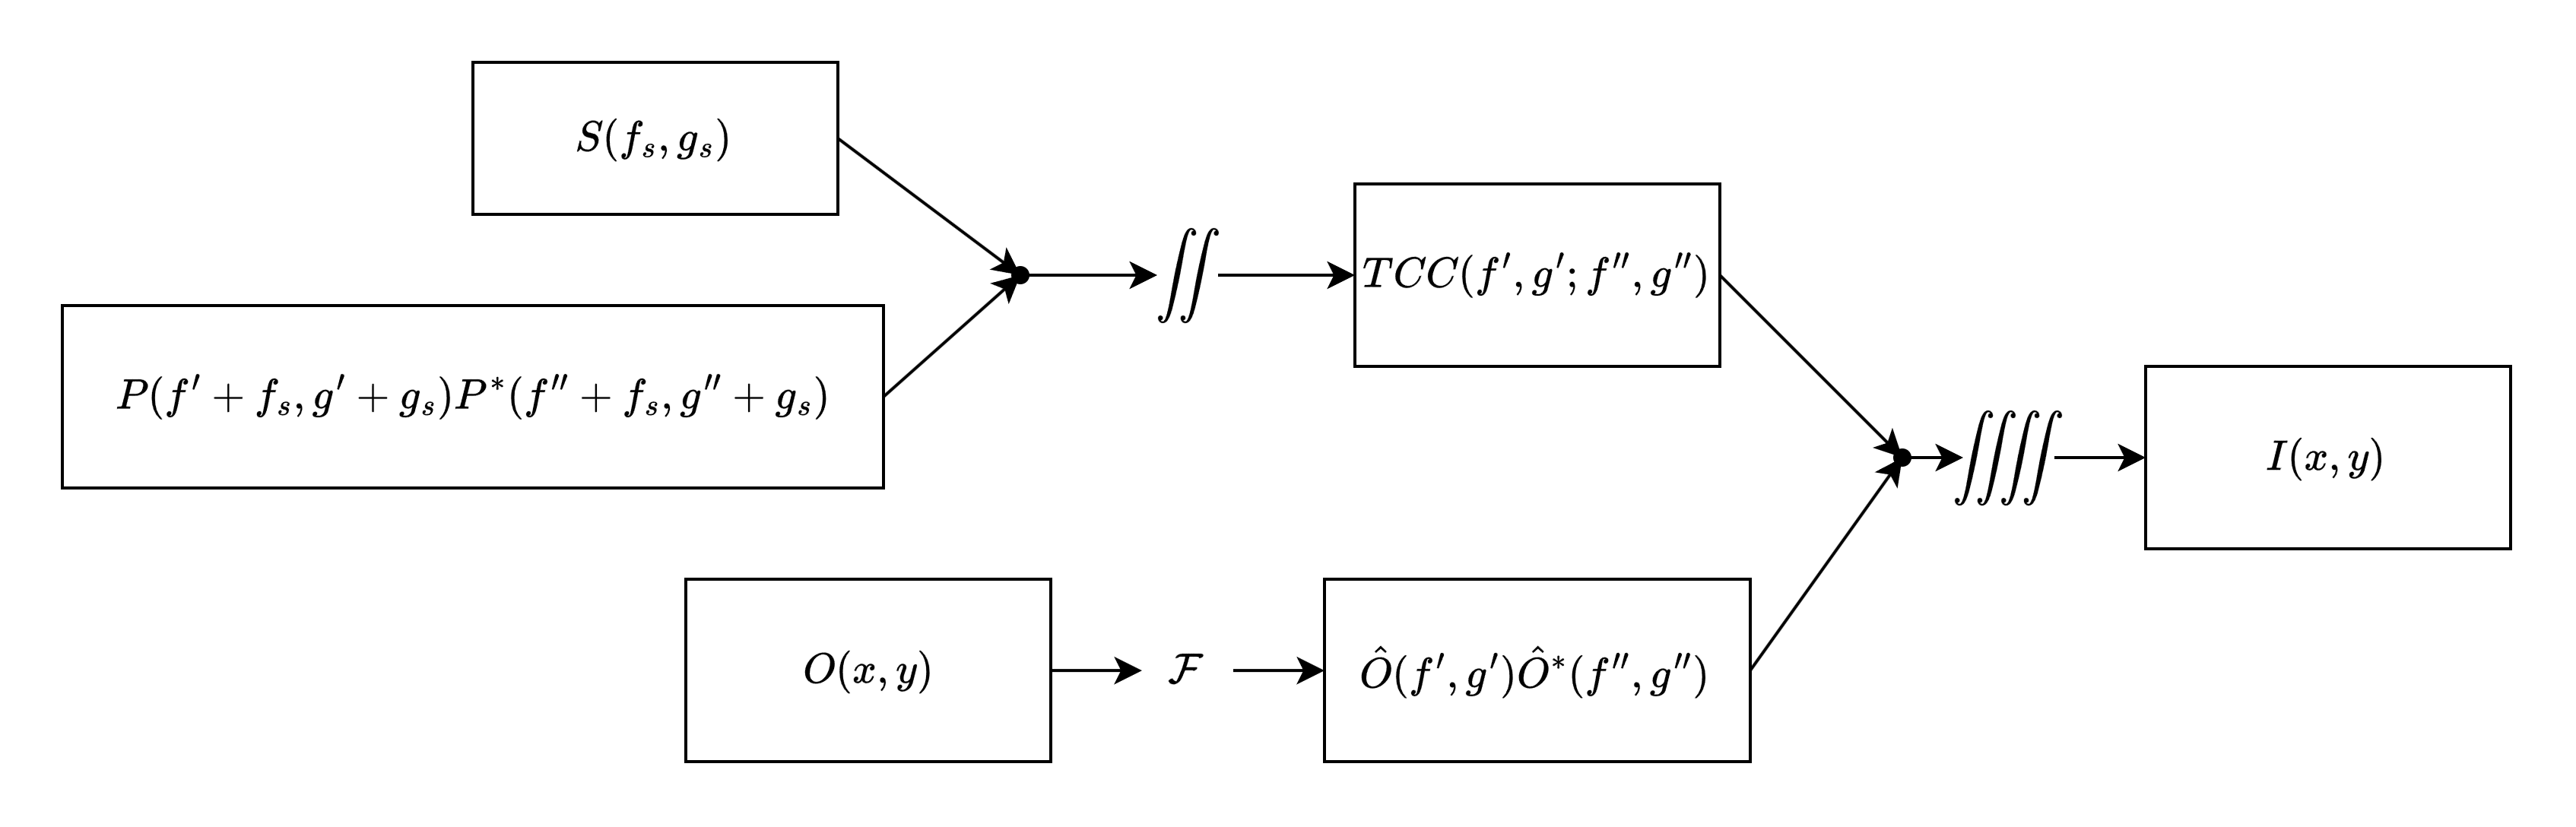
\includegraphics[keepaspectratio,alt={Figure 1 TCC-SOCS computational workflow}]{../image/论文/ch3_fig1_hopkins_workflow.png}}
\caption{Figure 1 TCC-SOCS computational workflow}
\end{figure}

\textbf{Figure 1} TCC-SOCS computational workflow. Offline
optical-system processing generates the SOCS eigenkernels and eigenvalue
weights, and the online reconstruction stage computes the aerial image
for each mask window.

Under the same offline optical model and online input conditions, the
computational paths of a conventional CPU-SOCS implementation and the
proposed decoupled CPU-FPGA architecture are shown in Fig. 2. Both
implementations share the SOCS eigenkernels and eigenvalue weights
generated offline and use the same mask spectrum and 10-kernel SOCS
imaging equation, ensuring that the architectural comparison is not
affected by differences in algorithmic configuration. The conventional
implementation reads data from host memory and sequentially executes ten
frequency-domain complex multiplications, FFTW two-dimensional IFFTs,
and intensity accumulations on the CPU. Its principal bottlenecks arise
from repeated software loops and memory accesses. In the proposed
architecture, the online inputs are transferred through PCIe to
FPGA-side DDR, and the frequently repeated computation is mapped to
three hardware stages: fixed-grid embedding, pipelined two-dimensional
IFFT, and on-chip intensity accumulation. The effective \(17 \times 17\)
frequency-domain data are embedded into a \(128 \times 128\) FFT grid, a
BRAM transpose buffer is placed between the row and column IFFTs, and
the inter-kernel accumulation result is retained in on-chip memory.
After computation, the \(128 \times 128\) result is read back through
PCIe and processed by host-side Fourier interpolation. The 35.6 ms and
10.57 ms values in the figure denote the CPU and FPGA kernel-only
latency, respectively, for the same 10-kernel online SOCS operator,
corresponding to a \(3.37\times\) kernel speedup. PCIe transfer and
host-side Fourier interpolation are excluded from this metric.

\begin{figure}
\centering
\pandocbounded{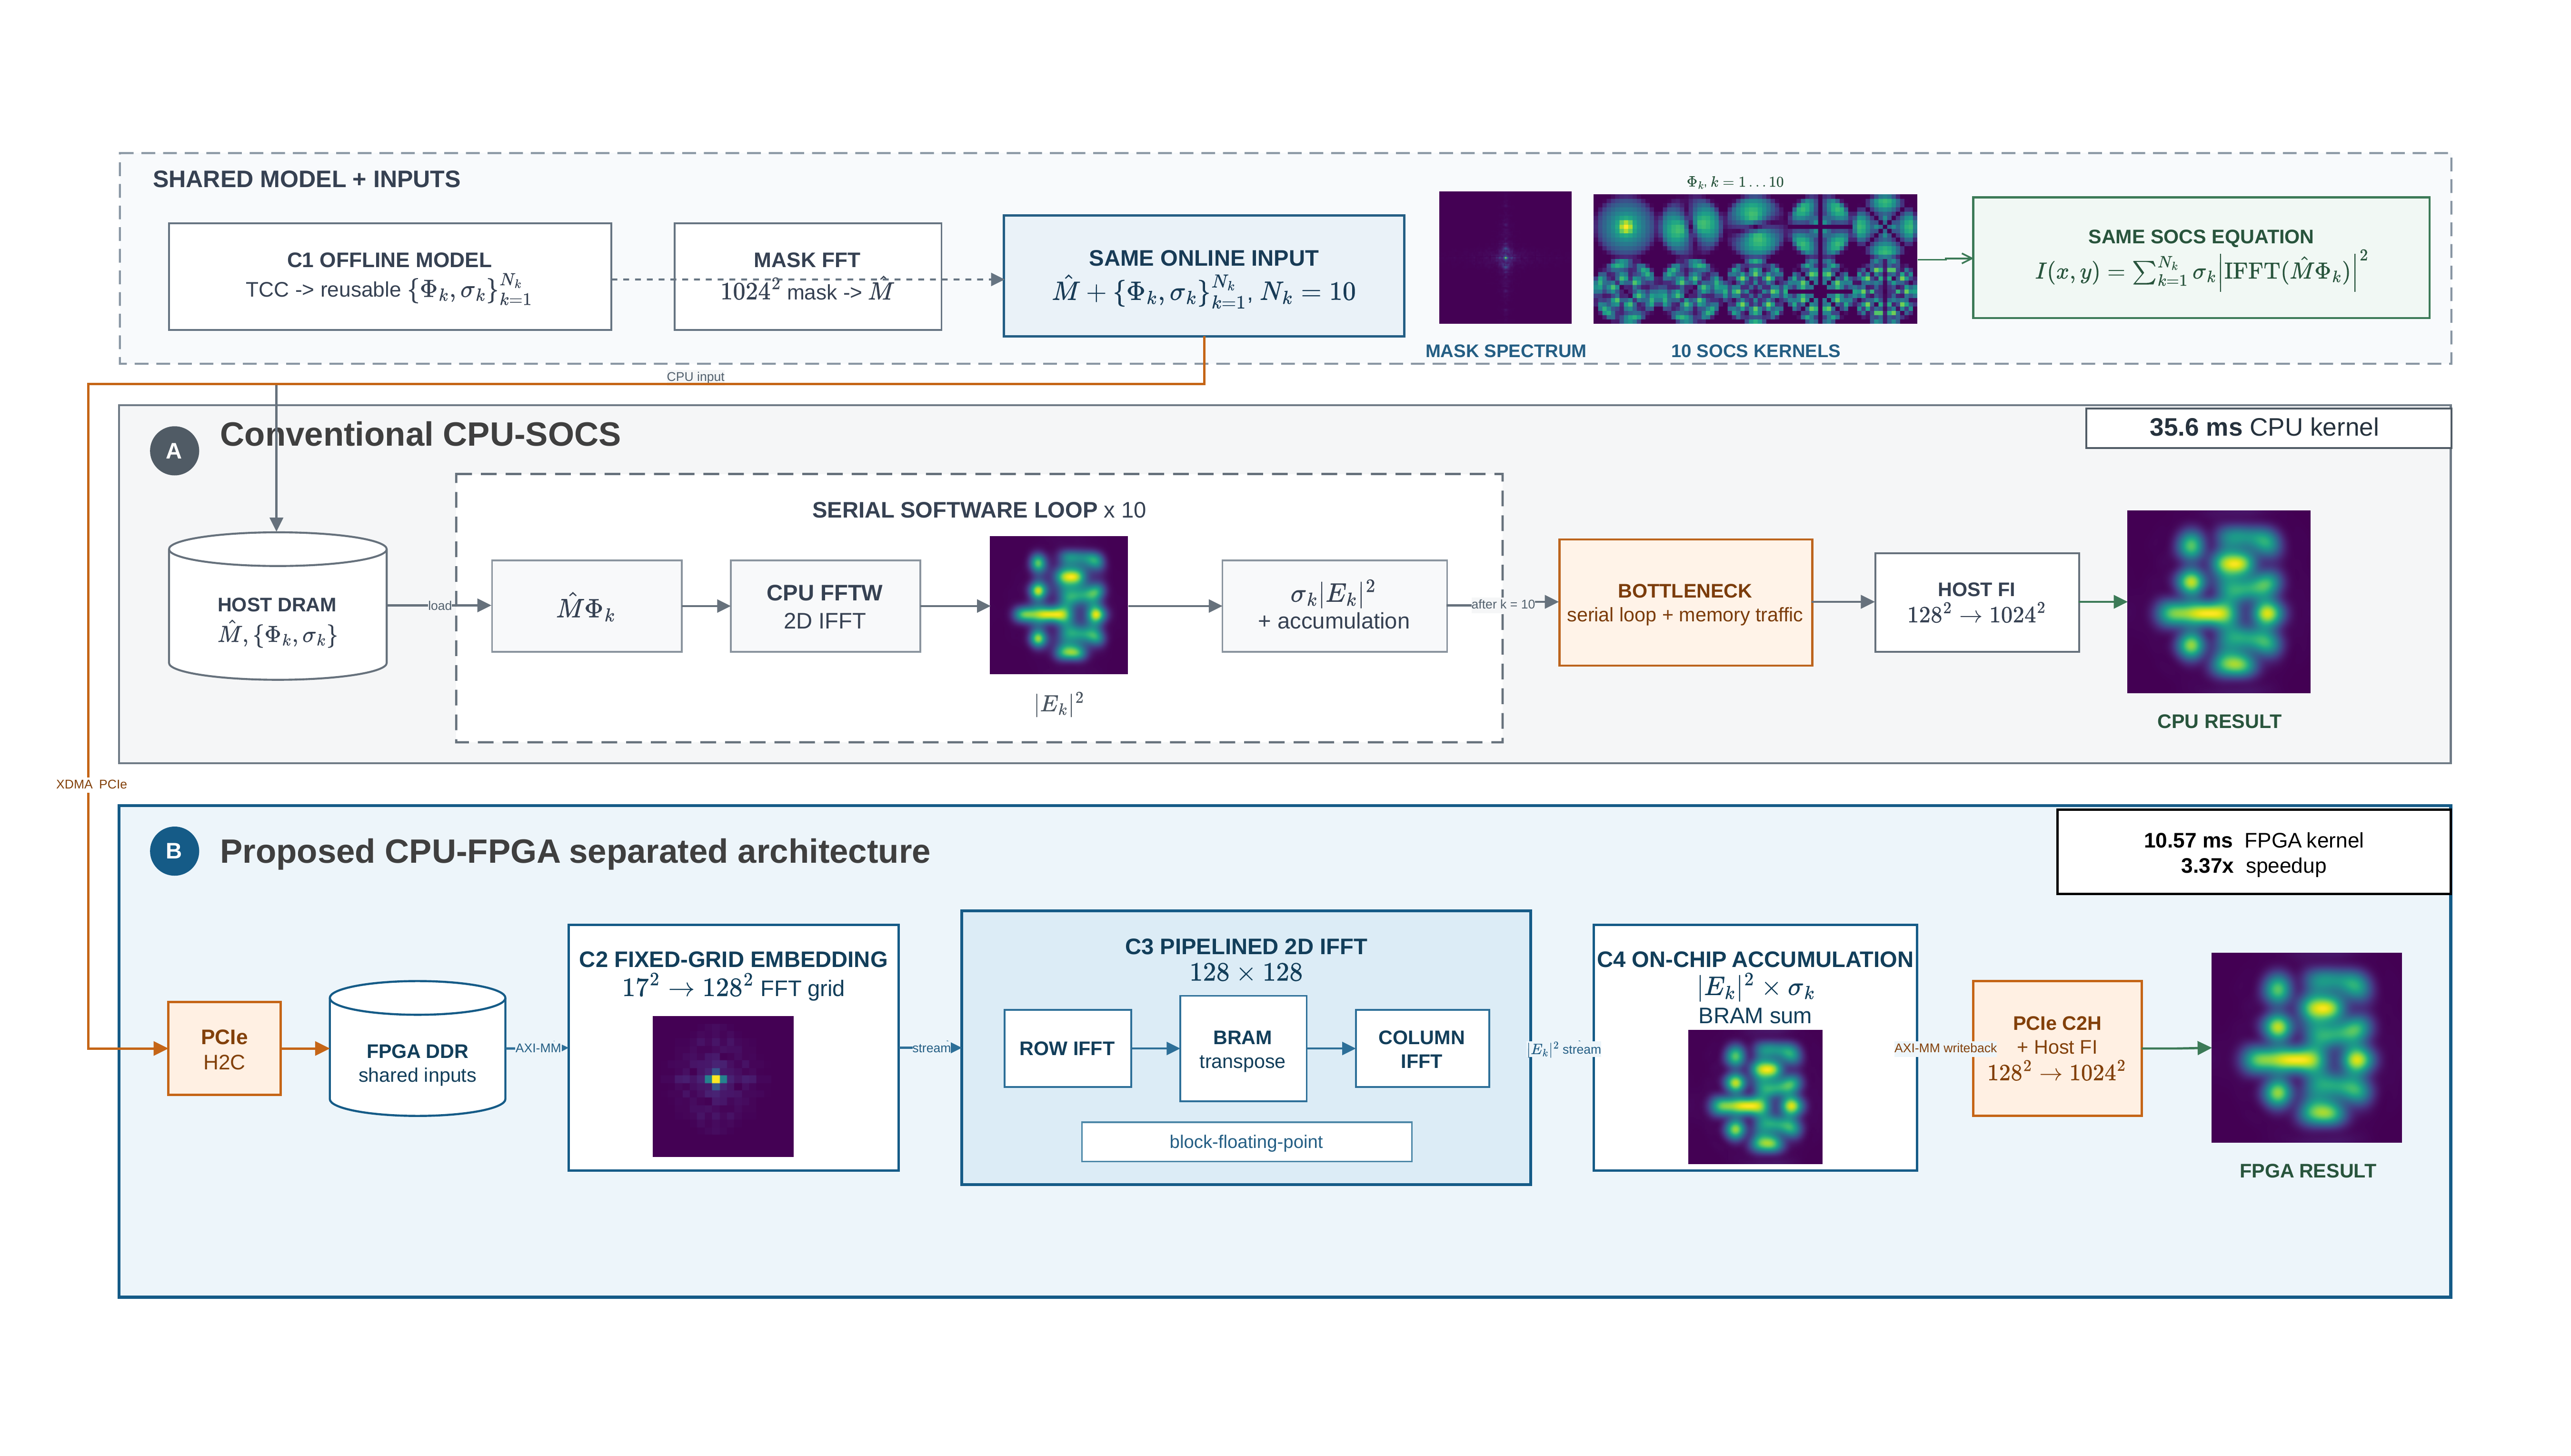
\includegraphics[keepaspectratio,alt={Figure 2 Comparison between conventional CPU-SOCS and the proposed decoupled CPU-FPGA architecture}]{../image/论文/fig2_cpu_fpga_socs_architecture_comparison.png}}
\caption{Figure 2 Comparison between conventional CPU-SOCS and the
proposed decoupled CPU-FPGA architecture}
\end{figure}

\textbf{Figure 2} Architectural comparison under the same SOCS model and
online inputs. (a) Conventional serial CPU-SOCS software path. (b)
Proposed decoupled CPU-FPGA architecture with fixed-grid embedding,
pipelined two-dimensional IFFT, and an on-chip accumulation datapath.
The latency and speedup shown are both reported on a kernel-only basis.

\textbf{Host-FPGA PCIe on-board validation flow.} The on-board system
uses Xilinx XDMA character devices for data transfers between the host
and FPGA. The host writes the real and imaginary parts of the
\(1024 \times 1024\) mask spectrum, the real and imaginary parts of ten
\(17 \times 17\) SOCS eigenkernels, and ten eigenvalue weights to
designated DDR addresses. It then writes \(N_k\), \(N_x\), \(N_y\),
\(L_x\), \(L_y\), and the buffer addresses through AXI-Lite registers
and asserts the start signal to launch the HLS IP. Upon completion, the
host reads back the scaled \(128 \times 128\) aerial image
\(I_{128\times128}\) and applies Fourier interpolation to obtain the
\(1024 \times 1024\) aerial image. This flow covers data writes, control
configuration, computation launch, result read-back, host
post-processing, and comparison with the reference result, thereby
validating system-level deployability.

\textbf{Table 2} Full-platform PCIe/XDMA data layout

{\def\LTcaptype{none} % do not increment counter
\begin{longtable}[]{@{}
  >{\raggedright\arraybackslash}p{(\linewidth - 10\tabcolsep) * \real{0.235}}
  >{\centering\arraybackslash}p{(\linewidth - 10\tabcolsep) * \real{0.080}}
  >{\raggedright\arraybackslash}p{(\linewidth - 10\tabcolsep) * \real{0.135}}
  >{\raggedright\arraybackslash}p{(\linewidth - 10\tabcolsep) * \real{0.175}}
  >{\raggedright\arraybackslash}p{(\linewidth - 10\tabcolsep) * \real{0.125}}
  >{\raggedright\arraybackslash}p{(\linewidth - 10\tabcolsep) * \real{0.250}}@{}}
\toprule\noalign{}
\begin{minipage}[b]{\linewidth}\raggedright
Data object
\end{minipage} & \begin{minipage}[b]{\linewidth}\raggedright
Direction
\end{minipage} & \begin{minipage}[b]{\linewidth}\raggedright
Address
\end{minipage} & \begin{minipage}[b]{\linewidth}\raggedright
Data volume
\end{minipage} & \begin{minipage}[b]{\linewidth}\raggedright
Data type
\end{minipage} & \begin{minipage}[b]{\linewidth}\raggedright
Description
\end{minipage} \\
\midrule\noalign{}
\endhead
\bottomrule\noalign{}
\endlastfoot
Real part of mask spectrum \(M_{\mathrm{Re}}\) & H2C &
\texttt{0x40000000} & 4,194,304 B & IEEE-754 single precision & Real
part of \(1024 \times 1024\) data \\
Imaginary part of mask spectrum \(M_{\mathrm{Im}}\) & H2C &
\texttt{0x40400000} & 4,194,304 B & IEEE-754 single precision &
Imaginary part of \(1024 \times 1024\) data \\
Eigenvalue weights \(\sigma_k\) & H2C & \texttt{0x40800000} & 40 B &
IEEE-754 single precision & 10 SOCS weights \\
Real parts of eigenkernels \(\Phi_{\mathrm{Re}}\) & H2C &
\texttt{0x40880000} & 11,560 B & IEEE-754 single precision & Real parts
of \(10 \times 17 \times 17\) data \\
Imaginary parts of eigenkernels \(\Phi_{\mathrm{Im}}\) & H2C &
\texttt{0x40900000} & 11,560 B & IEEE-754 single precision & Imaginary
parts of \(10 \times 17 \times 17\) data \\
Intermediate accumulated image \(I_{\mathrm{acc}}\) & H2C &
\texttt{0x40980000} & 65,536 B, zero initialized & IEEE-754 single
precision & \(128 \times 128\) accumulation buffer \\
Output image \(I_{128\times128}\) & H2C & \texttt{0x40990000} & 65,536
B, zero initialized & IEEE-754 single precision & \(128 \times 128\)
output buffer \\
FPGA output \(I_{128\times128}\) & C2H & \texttt{0x40990000} & 65,536 B
& IEEE-754 single precision & Host FI to \(1024 \times 1024\) after
read-back \\
\end{longtable}
}

\textbf{FPGA online reconstruction pipeline.} The FPGA pipeline
comprises five stages:

\begin{enumerate}
\def\labelenumi{\arabic{enumi}.}
\tightlist
\item
  \textbf{Frequency-domain embedding:} The SOCS eigenkernel is
  multiplied by the corresponding central window of the mask spectrum,
  and the product is embedded into a fixed \(128 \times 128\) FFT grid.
\item
  \textbf{Two-dimensional IFFT:} A block-floating-point two-dimensional
  complex IFFT processor sequentially performs row-wise FFT,
  conflict-free matrix transposition, and column-wise FFT.
\item
  \textbf{Weighted accumulation:} \(|E_k|^2\) is evaluated, and
  \(\sigma_k|E_k|^2\) is accumulated in a temporary image buffer.
\item
  \textbf{FFTshift:} Quadrant exchange moves the zero-frequency
  component to the image center.
\item
  \textbf{Output write-back:} The final \(128 \times 128\) image is
  written back to DDR through AXI-MM burst accesses.
\end{enumerate}

In terms of data dependencies, the online stage requires only the mask
spectrum, SOCS eigenkernels, and eigenvalue weights. Optical information
such as the source, pupil, and aberrations has already been compressed
into \(\Phi_k\) and \(\sigma_k\) during the offline stage. For the
\(k\)th eigenkernel, the FPGA first performs pointwise complex
multiplication between the mask spectrum and the eigenkernel within the
effective frequency-domain window, and centrally embeds the result into
the \(128 \times 128\) frequency grid:

\[
F_k(c_x+u,c_y+v)=M(c_x+u,c_y+v)\Phi_k(u,v),
\quad |u|\leq N_x,\ |v|\leq N_y .
\tag{7}
\]

The two-dimensional IFFT then produces the coherent field \(E_k\), whose
intensity \(|E_k|^2\) is weighted by \(\sigma_k\) and accumulated in the
output buffer. After all retained eigenkernels have been processed, the
hardware applies FFTshift to the accumulated image and writes it back to
external memory. The online FPGA stage can therefore be expressed as

\[
\hat{I}=\mathrm{FFTshift}\left(\sum_{k=1}^{N_k}\sigma_k
\left|\mathcal{F}^{-1}\{F_k\}\right|^2\right).
\tag{8}
\]

Under the default 10-kernel configuration, the five-stage path is
executed sequentially for each eigenkernel. This inter-kernel
time-multiplexing strategy reuses a single two-dimensional IFFT engine
across multiple eigenkernels, avoiding excessive BRAM consumption.
Although fully parallel kernel processing could provide higher
throughput, each parallel kernel would require an independent
\(128 \times 128\) two-dimensional IFFT instance and transpose buffer.
Based on the resource model of the current HLS FFT IP, full parallelism
across ten kernels would require approximately 3000 BRAM\_18K blocks,
about 3.1 times the 960 BRAM\_18K blocks available on the xcku5p. This
work therefore adopts a compromise combining inter-kernel time
multiplexing with intra-kernel pipelining.

The host configures the number of kernels \(N_k\), effective
frequency-domain extent \(N_x,N_y\), mask dimensions \(L_x,L_y\), and
AXI-MM pointer addresses through the AXI-Lite interface. With a fixed
\(128 \times 128\) IFFT grid, different effective kernel sizes can reuse
the same hardware configuration through zero padding and central
embedding, thereby avoiding repeated synthesis for different optical
configurations.

\subsection{2.3 Key Hardware Modules and Memory
Architecture}\label{key-hardware-modules-and-memory-architecture}

This section summarizes the three design components that determine
performance and resource consumption: frequency-domain embedding,
two-dimensional IFFT, and memory access. Under the default
configuration, the effective eigenkernel size is \(17 \times 17\),
corresponding to \(N_x=N_y=8\). Referenced to the center of the mask
spectrum \((L_x/2,L_y/2)\), the embedding module performs pointwise
complex multiplication over the central window, maps the result into the
fixed \(128 \times 128\) frequency grid, and zero pads the remaining
positions. This organization preserves the frequency ordering and
spatial phase of the FPGA output relative to the CPU reference. The
embedding loop uses \texttt{PIPELINE\ II=1}; runtime parameters \(N_x\)
and \(N_y\) define the effective window, with \(17 \times 17\) as the
synthesis bound.

The control interface receives runtime parameters including \(N_k\),
\(N_x\), \(N_y\), \(L_x\), and \(L_y\). The mask spectrum, eigenkernels,
weights, intermediate image, and output image are mapped to independent
AXI-MM access channels. Initialization, frequency-domain embedding,
intensity accumulation, and result write-back are pipelined, while the
two-dimensional intermediate matrices and accumulation buffers are bound
to dual-port BRAM to reduce repeated accesses to external DDR.

\textbf{Two-dimensional IFFT engine.} The dominant computation is
implemented by time-multiplexing one \(128 \times 128\) two-dimensional
IFFT datapath across the SOCS eigenkernels. Separate real and imaginary
dual-port BRAMs provide conflict-free transpose buffering between the
row and column transforms, avoiding additional DDR round trips. The
underlying 128-point one-dimensional FFT uses natural-order output,
block-floating-point scaling, LUT-mapped multiplication, and
\texttt{ap\_fixed\textless{}32,1\textgreater{}} input and output. The
row and column scaling exponents are accumulated and compensated jointly
during fixed-to-floating-point conversion:

\[
E_{\mathrm{float}}=E_{\mathrm{fixed}}\cdot 2^{\mathrm{blk\_exp}}.
\qquad\mathrm{(9)}
\]

Compared with a fixed right shift at every stage, this strategy reduces
accumulated scaling error and lowers DSP utilization by mapping
butterfly multiplications to LUTs. The limited BRAM capacity is
therefore prioritized for transpose and accumulation buffers while the
SOCS imaging model remains unchanged.

\textbf{Memory architecture.} The top-level HLS IP uses seven
independent AXI-MM master interfaces:

{\def\LTcaptype{none} % do not increment counter
\begin{longtable}[]{@{}
  >{\raggedright\arraybackslash}p{(\linewidth - 8\tabcolsep) * \real{0.0800}}
  >{\raggedright\arraybackslash}p{(\linewidth - 8\tabcolsep) * \real{0.2800}}
  >{\raggedright\arraybackslash}p{(\linewidth - 8\tabcolsep) * \real{0.3000}}
  >{\raggedleft\arraybackslash}p{(\linewidth - 8\tabcolsep) * \real{0.1800}}
  >{\raggedright\arraybackslash}p{(\linewidth - 8\tabcolsep) * \real{0.1600}}@{}}
\toprule\noalign{}
\begin{minipage}[b]{\linewidth}\raggedright
Channel
\end{minipage} & \begin{minipage}[b]{\linewidth}\raggedright
Data channel
\end{minipage} & \begin{minipage}[b]{\linewidth}\raggedright
Data
\end{minipage} & \begin{minipage}[b]{\linewidth}\raggedleft
Depth
\end{minipage} & \begin{minipage}[b]{\linewidth}\raggedright
Access mode
\end{minipage} \\
\midrule\noalign{}
\endhead
\bottomrule\noalign{}
\endlastfoot
0 & Real part of mask spectrum & Real part of mask spectrum & 1,048,576
& Read \\
1 & Imaginary part of mask spectrum & Imaginary part of mask spectrum &
1,048,576 & Read \\
2 & Eigenvalue weights & SOCS eigenvalue weights & 32 & Read \\
3 & Real parts of eigenkernels & Real parts of eigenkernels & 76,832 &
Read \\
4 & Imaginary parts of eigenkernels & Imaginary parts of eigenkernels &
76,832 & Read \\
5 & Intermediate image buffer & Intermediate image & 16,384 & Write \\
6 & Final image buffer & Final image & 16,384 & Write \\
\end{longtable}
}

The principal on-chip buffers are bound to BRAM to reduce repeated DDR
accesses during FFT and accumulation. This memory organization separates
large streaming inputs, small scalar parameters, and output buffers,
thereby reducing bus congestion and improving burst-access efficiency.

For reproducibility, Table 3 lists the key HLS and interface
configurations. All external DDR data use IEEE-754 single-precision
floating point, whereas the FFT IP internally uses the
\texttt{ap\_fixed\textless{}32,1\textgreater{}} complex fixed-point
format. In block-floating-point mode, \texttt{blk\_exp} records the
total scaling and compensates the floating-point result according to Eq.
(9).

\textbf{Table 3} Key HLS/IP implementation configurations

{\def\LTcaptype{none} % do not increment counter
\begin{longtable}[]{@{}
  >{\raggedright\arraybackslash}p{(\linewidth - 2\tabcolsep) * \real{0.5000}}
  >{\raggedright\arraybackslash}p{(\linewidth - 2\tabcolsep) * \real{0.5000}}@{}}
\toprule\noalign{}
\begin{minipage}[b]{\linewidth}\raggedright
Category
\end{minipage} & \begin{minipage}[b]{\linewidth}\raggedright
Configuration
\end{minipage} \\
\midrule\noalign{}
\endhead
\bottomrule\noalign{}
\endlastfoot
Top-level module & TCC-SOCS online reconstruction HLS kernel \\
FFT IP & Fixed length of 128 points, \(\log_2 N=7\), single channel,
pipelined streaming I/O, and natural-order output \\
FFT numerical format & Input/output
\texttt{ap\_fixed\textless{}32,1\textgreater{}}; 32-bit two's-complement
fixed point with a 1-bit integer width and 31-bit fractional precision;
phase factor width of 24; block-floating-point scaling; truncation
rounding \\
FFT storage and multiplication & BRAM for data, twiddle-factor, and
reordering storage; complex and butterfly multiplications mapped to
LUTs \\
Main loop optimizations & \texttt{PIPELINE\ II=1} applied to
frequency-grid initialization, embedding, intensity accumulation,
FFTshift, format conversion, and DDR write-back loops \\
Kernel-loop constraint & Default synthesis bound of 10 SOCS kernels with
runtime configuration of the kernel count \\
On-chip buffers & Input/output complex buffers, accumulated-image
buffer, scaled-image buffer, and intermediate FFT transpose buffers
bound to dual-port BRAM \\
AXI-MM read channels & Burst length 64 and 8 outstanding transactions
for real/imaginary mask-spectrum reads; burst length 32 and 4
outstanding transactions for real/imaginary eigenkernel reads \\
AXI-MM write channels & Burst length 64 and 4 outstanding transactions
for intermediate accumulated-image and output-image writes \\
AXI-Lite control & \(N_k\), \(N_x\), \(N_y\), \(L_x\), \(L_y\), and all
AXI-MM pointer addresses configured by the host \\
\end{longtable}
}

\section{3. Simulation and
Experiments}\label{simulation-and-experiments}

\subsection{3.1 Experimental Configuration and Evaluation
Scope}\label{experimental-configuration-and-evaluation-scope}

A representative DUV configuration is fixed throughout the experiments
to prevent variations in parameter combinations from confounding the
platform comparison. The target FPGA is a Xilinx Kintex UltraScale+
xcku5p-ffvb676-2-e. The design is implemented using Vitis HLS 2025.2 and
Vivado 2025.2, and all timing results are evaluated at 250 MHz. The
software performance baseline runs on an Intel Xeon Platinum 8163
server. The C++ program uses C++17, single-precision floating point, and
\texttt{-O2} optimization, and links against FFTW 3.x, LAPACK, BLAS, and
OpenMP runtime libraries. Table 4 summarizes the experimental
configuration.

\textbf{Table 4} Fixed experimental configuration and comparison scope

{\def\LTcaptype{none} % do not increment counter
\begin{longtable}[]{@{}
  >{\raggedright\arraybackslash}p{(\linewidth - 2\tabcolsep) * \real{0.3333}}
  >{\raggedright\arraybackslash}p{(\linewidth - 2\tabcolsep) * \real{0.6667}}@{}}
\toprule\noalign{}
\begin{minipage}[b]{\linewidth}\raggedright
Category
\end{minipage} & \begin{minipage}[b]{\linewidth}\raggedright
Fixed configuration
\end{minipage} \\
\midrule\noalign{}
\endhead
\bottomrule\noalign{}
\endlastfoot
Optics and input & \(L_x=L_y=1024\), \(NA=0.8\), \(\lambda=193\) nm,
annular source, \(\sigma_{in}=0.6\), \(\sigma_{out}=0.9\) \\
SOCS configuration & Ten \(17\times17\) eigenkernels and a fixed
\(128\times128\) FFT grid \\
FPGA & xcku5p-ffvb676-2-e, Vitis HLS/Vivado 2025.2, 250 MHz \\
CPU baseline & Intel Xeon Platinum 8163 @ 2.50 GHz, GCC 13.3.0, C++17,
single precision, \texttt{-O2} \\
Accuracy reference & Full MATLAB TCC and high-precision 10-kernel SOCS
results \\
Performance baseline & C++ 10-kernel SOCS online reconstruction using
the same input and imaging equation as the FPGA \\
\end{longtable}
}

Accuracy and performance are evaluated against distinct but
complementary references. MATLAB is used to quantify the model
truncation error of the 10-kernel SOCS approximation relative to the
full TCC. The SOCS software Golden result under the same configuration
is used to isolate the hardware implementation error caused by FPGA
fixed-point quantization, block-floating-point scaling, and data-format
conversion. The speedup compares only the same 10-kernel online SOCS
operator on the C++ CPU and FPGA, excluding offline TCC construction,
eigendecomposition, PCIe transfer, and host-side Fourier interpolation.

\subsection{3.2 Accuracy Validation Against
MATLAB}\label{accuracy-validation-against-matlab}

Given an image under validation \(X\) and a reference image \(Y\), the
root mean square error is used to quantify the overall deviation:

\[
\mathrm{RMSE}(X,Y)=\sqrt{\frac{1}{N}\sum_{i=1}^{N}(X_i-Y_i)^2}.
\qquad\mathrm{(10)}
\]

Table 5 reports the model truncation error and hardware implementation
error separately. The RMSE between the MATLAB 10-kernel SOCS result and
direct full-TCC imaging is \(5.472\times10^{-3}\), with a PSNR of 36.95
dB and a binary-pattern agreement of 98.77\%. This result establishes
the error bound of the fixed 10-kernel model relative to the
high-precision physical reference. The on-board \(128\times128\) FPGA
output has an RMSE of \(2.93\times10^{-8}\) relative to the SOCS
software Golden result under the same configuration. After host-side
Fourier interpolation recovers the \(1024\times1024\) image, the RMSE is
\(2.95\times10^{-8}\) and the PSNR is 142.20 dB.

\textbf{Table 5} Accuracy validation results under the fixed 10-kernel
configuration

{\def\LTcaptype{none} % do not increment counter
\begin{longtable}[]{@{}
  >{\raggedright\arraybackslash}p{(\linewidth - 8\tabcolsep) * \real{0.250}}
  >{\raggedright\arraybackslash}p{(\linewidth - 8\tabcolsep) * \real{0.310}}
  >{\raggedleft\arraybackslash}p{(\linewidth - 8\tabcolsep) * \real{0.145}}
  >{\raggedleft\arraybackslash}p{(\linewidth - 8\tabcolsep) * \real{0.155}}
  >{\raggedleft\arraybackslash}p{(\linewidth - 8\tabcolsep) * \real{0.140}}@{}}
\toprule\noalign{}
\begin{minipage}[b]{\linewidth}\raggedright
Result under validation
\end{minipage} & \begin{minipage}[b]{\linewidth}\raggedright
Reference
\end{minipage} & \begin{minipage}[b]{\linewidth}\raggedleft
RMSE
\end{minipage} & \begin{minipage}[b]{\linewidth}\raggedleft
MaxAE
\end{minipage} & \begin{minipage}[b]{\linewidth}\raggedleft
PSNR
\end{minipage} \\
\midrule\noalign{}
\endhead
\bottomrule\noalign{}
\endlastfoot
MATLAB 10-kernel SOCS & Full MATLAB TCC & \(5.472\times10^{-3}\) &
\(9.821\times10^{-3}\) & 36.95 dB \\
On-board FPGA \(128\times128\) output & SOCS software Golden under the
same configuration & \(2.93\times10^{-8}\) & \(3.58\times10^{-7}\) &
142.26 dB \\
FPGA+Host FI \(1024\times1024\) output & SOCS software Golden under the
same configuration & \(2.95\times10^{-8}\) & \(4.17\times10^{-7}\) &
142.20 dB \\
\end{longtable}
}

The FPGA hardware implementation error is approximately five orders of
magnitude smaller than the model truncation error of the 10-kernel SOCS
approximation. Thus, the deviation of the final aerial image from the
full MATLAB TCC result is governed primarily by low-rank truncation
rather than the FPGA datapath. C/RTL co-simulation gives an RMSE of
\(8.324\times10^{-7}\), which is also below the hardware implementation
error threshold of \(10^{-5}\). Figure 3 shows the reference image, FPGA
output, and error distribution under the fixed configuration; the
principal imaging structures are preserved in both images.

\begin{figure}
\centering
\pandocbounded{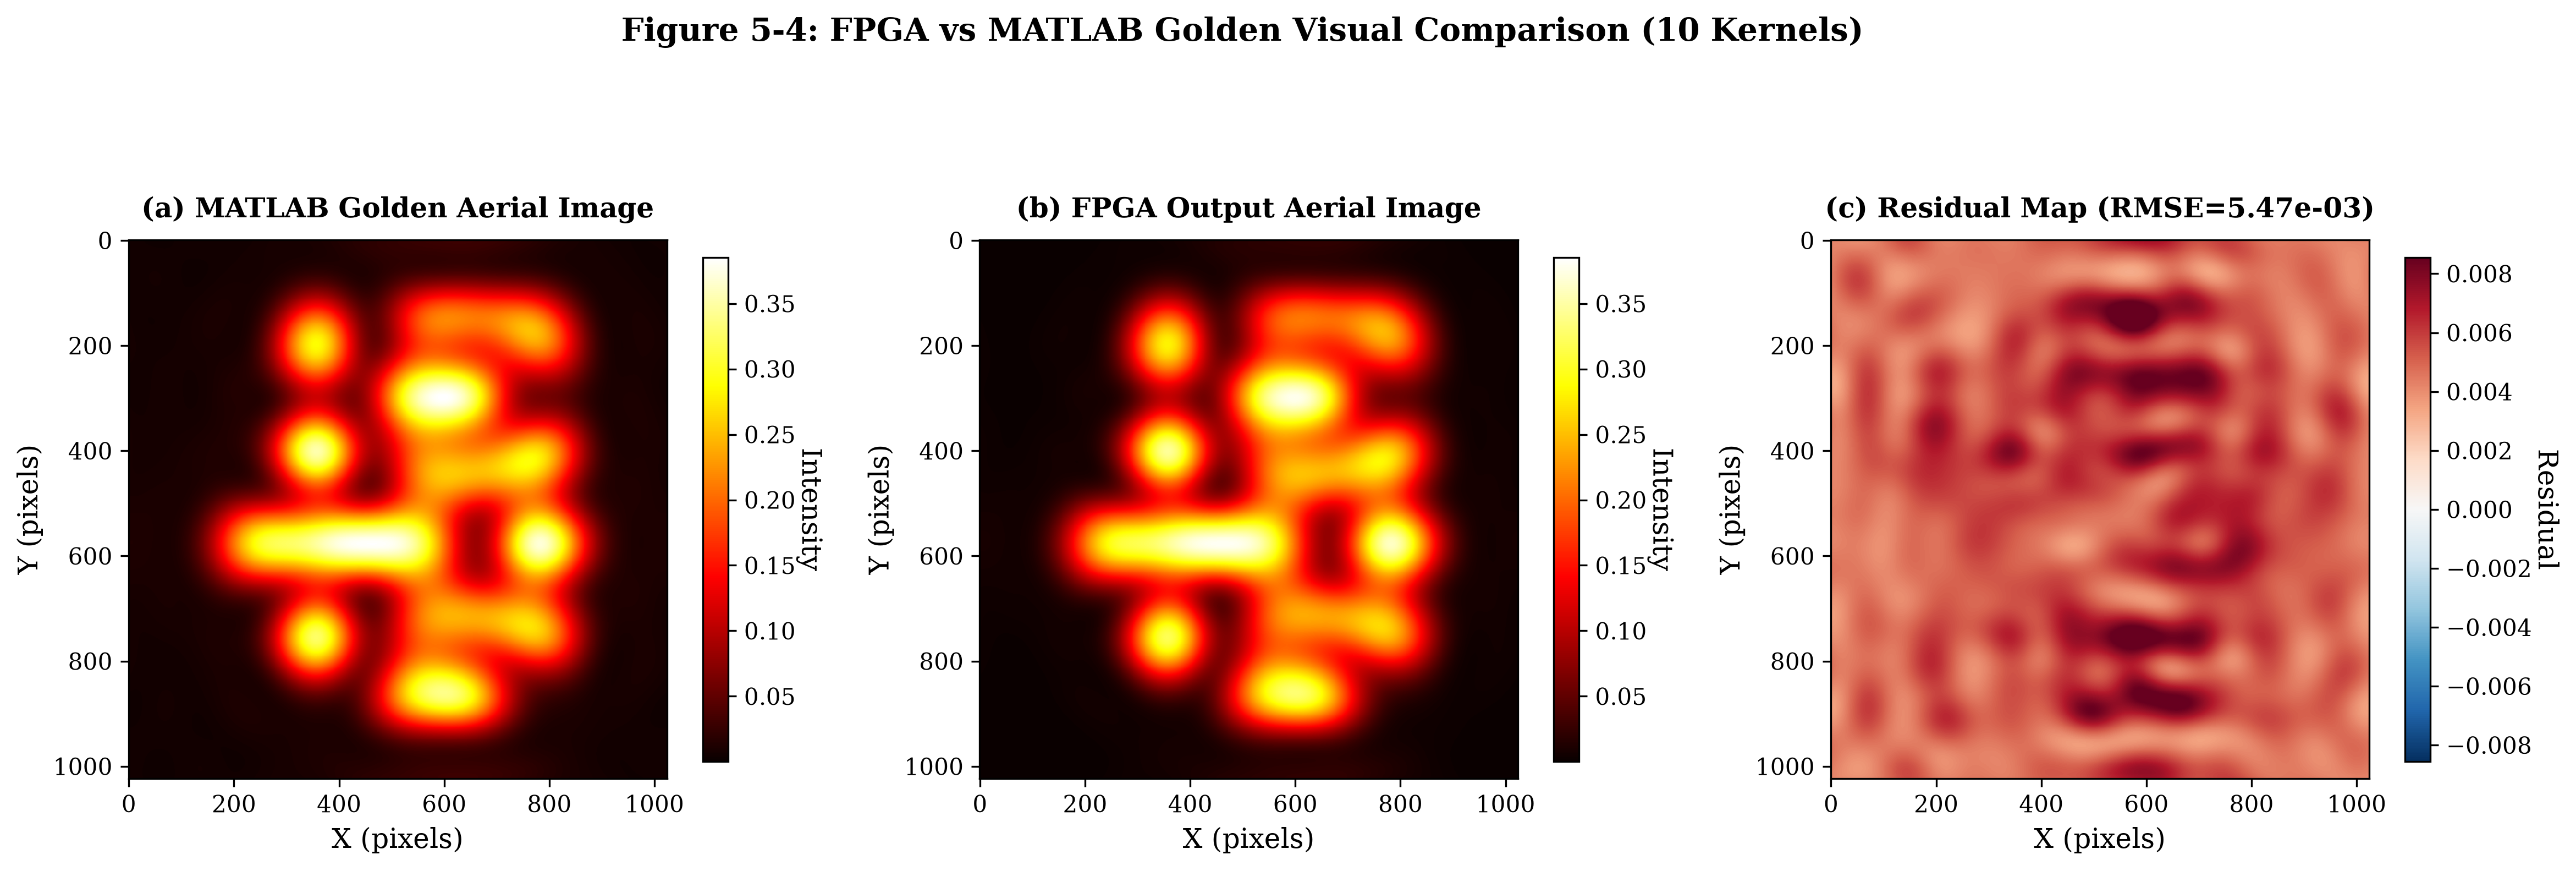
\includegraphics[keepaspectratio,alt={Figure 3 Visual comparison between the reference result and FPGA output under the fixed 10-kernel configuration}]{../image/论文/ch5_fig4_visual_comparison.png}}
\caption{Figure 3 Visual comparison between the reference result and
FPGA output under the fixed 10-kernel configuration}
\end{figure}

\textbf{Figure 3} Reference aerial image, FPGA output, and error
distribution under the fixed 10-kernel configuration. The full-TCC
result illustrates the model truncation error, whereas the hardware
implementation error is evaluated against the SOCS software Golden
result under the same configuration, as reported in Table 5.

Further on-board validation was performed using ten different layout
samples, all of which passed the accuracy checks. Relative to the SOCS
software Golden result under the same configuration, the FPGA+Host FI
output achieved an average RMSE of \(2.65\times10^{-8}\) and a
worst-case RMSE of \(3.58\times10^{-8}\). The average SSIM was
0.999999995, and the binary-pattern agreement at a threshold of 0.225
was 100\% for every sample. Figure 4 compares the input masks with their
corresponding on-board reconstruction results.

\begin{figure}
\centering
\pandocbounded{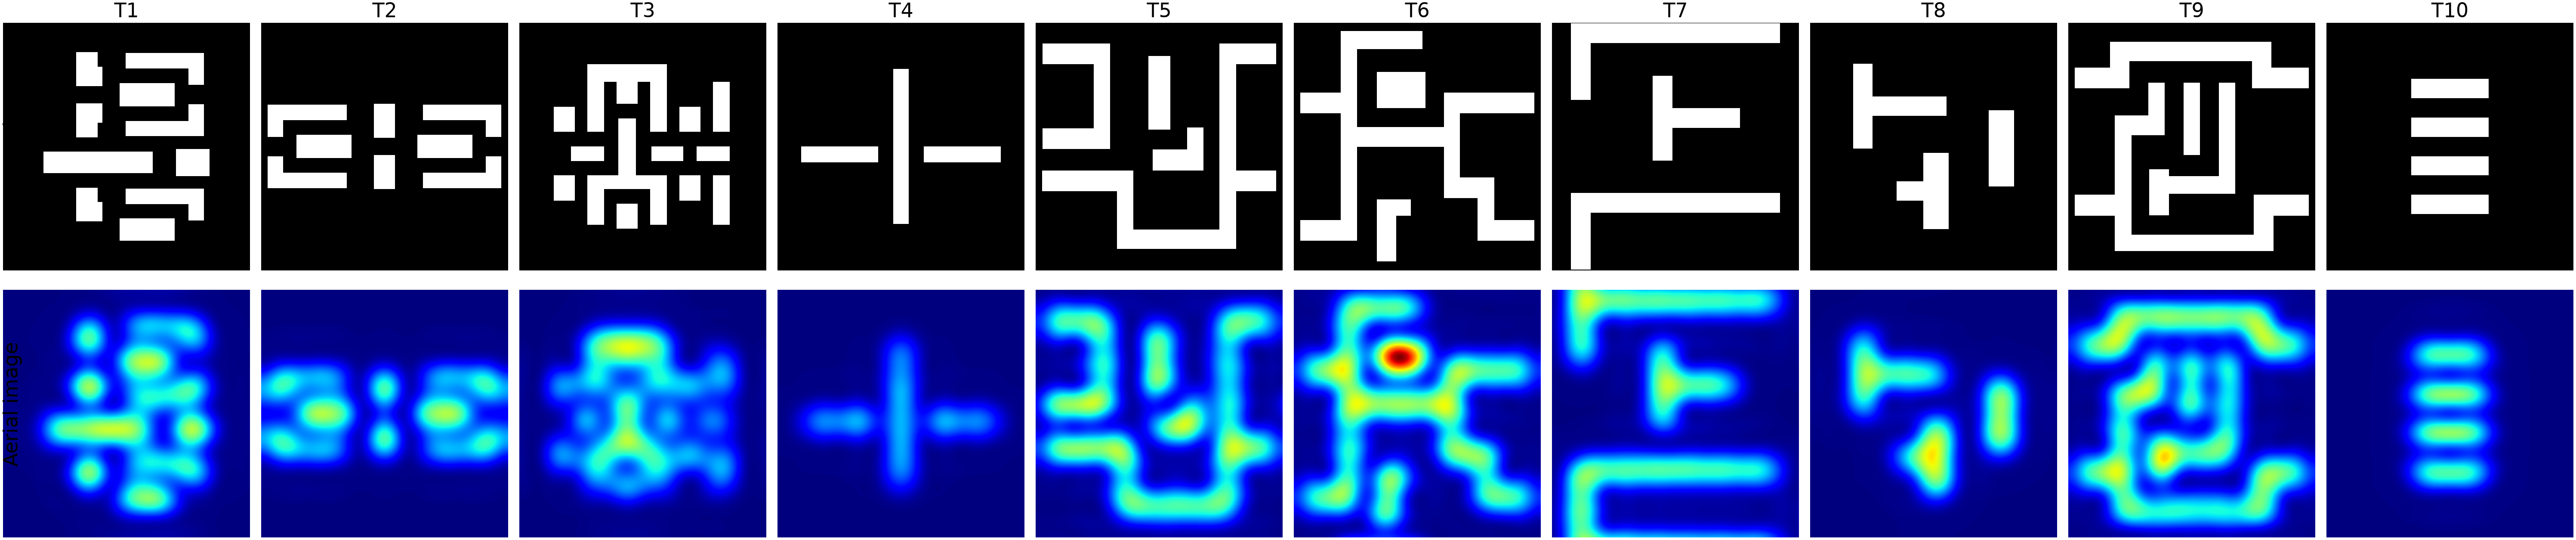
\includegraphics[keepaspectratio,alt={Figure 4 On-board aerial image reconstruction results for ten different mask samples}]{../image/论文/multi_mask_fpga_results.png}}
\caption{Figure 4 On-board aerial image reconstruction results for ten
different mask samples}
\end{figure}

\textbf{Figure 4} Input masks and FPGA+Host FI reconstruction results
for ten different mask samples, T1--T10. The upper row shows the input
masks, and the lower row shows the corresponding aerial images by
column.

\subsection{3.3 Speedup and Energy-Efficiency
Analysis}\label{speedup-and-energy-efficiency-analysis}

\subsubsection{3.3.1 FPGA Kernel Latency}\label{fpga-kernel-latency}

At 250 MHz, the top-level latency reported by HLS synthesis is 2,643,645
cycles, corresponding to 10.57 ms. C/RTL co-simulation reports 2,651,856
cycles, corresponding to 10.61 ms. The difference is approximately
0.3\%, indicating that the synthesis estimate is representative of the
execution cycles of the generated RTL. Table 6 provides a stage-wise
breakdown of the FPGA kernel.

\textbf{Table 6} Latency breakdown of the 10-kernel SOCS online
reconstruction kernel. Kernel-only latency at 250 MHz is reported; PCIe
transfer and host FI are excluded.

{\def\LTcaptype{none} % do not increment counter
\begin{longtable}[]{@{}lrrr@{}}
\toprule\noalign{}
Stage & Cycles & Time at 250 MHz & Proportion \\
\midrule\noalign{}
\endhead
\bottomrule\noalign{}
\endlastfoot
Frequency-domain embedding, 10 kernels & 167,450 & 0.67 ms & 6.3\% \\
Two-dimensional IFFT, 10 kernels & 2,262,250 & 9.05 ms & 85.6\% \\
Accumulation, 10 kernels & 164,250 & 0.66 ms & 6.2\% \\
FFTshift & 16,389 & 0.066 ms & 0.6\% \\
DDR output & 16,389 & 0.066 ms & 0.6\% \\
\textbf{Total} & \textbf{2,643,645} & \textbf{10.57 ms} &
\textbf{100\%} \\
\end{longtable}
}

The two-dimensional IFFT accounts for 85.6\% of the total latency and is
the principal performance bottleneck in the current online
reconstruction kernel. Frequency-domain embedding and intensity
accumulation account for only 6.3\% and 6.2\%, respectively. Fixed-grid
reuse, on-chip transposition, and IFFT-datapath optimization therefore
directly determine the overall latency.

\begin{figure}
\centering
\pandocbounded{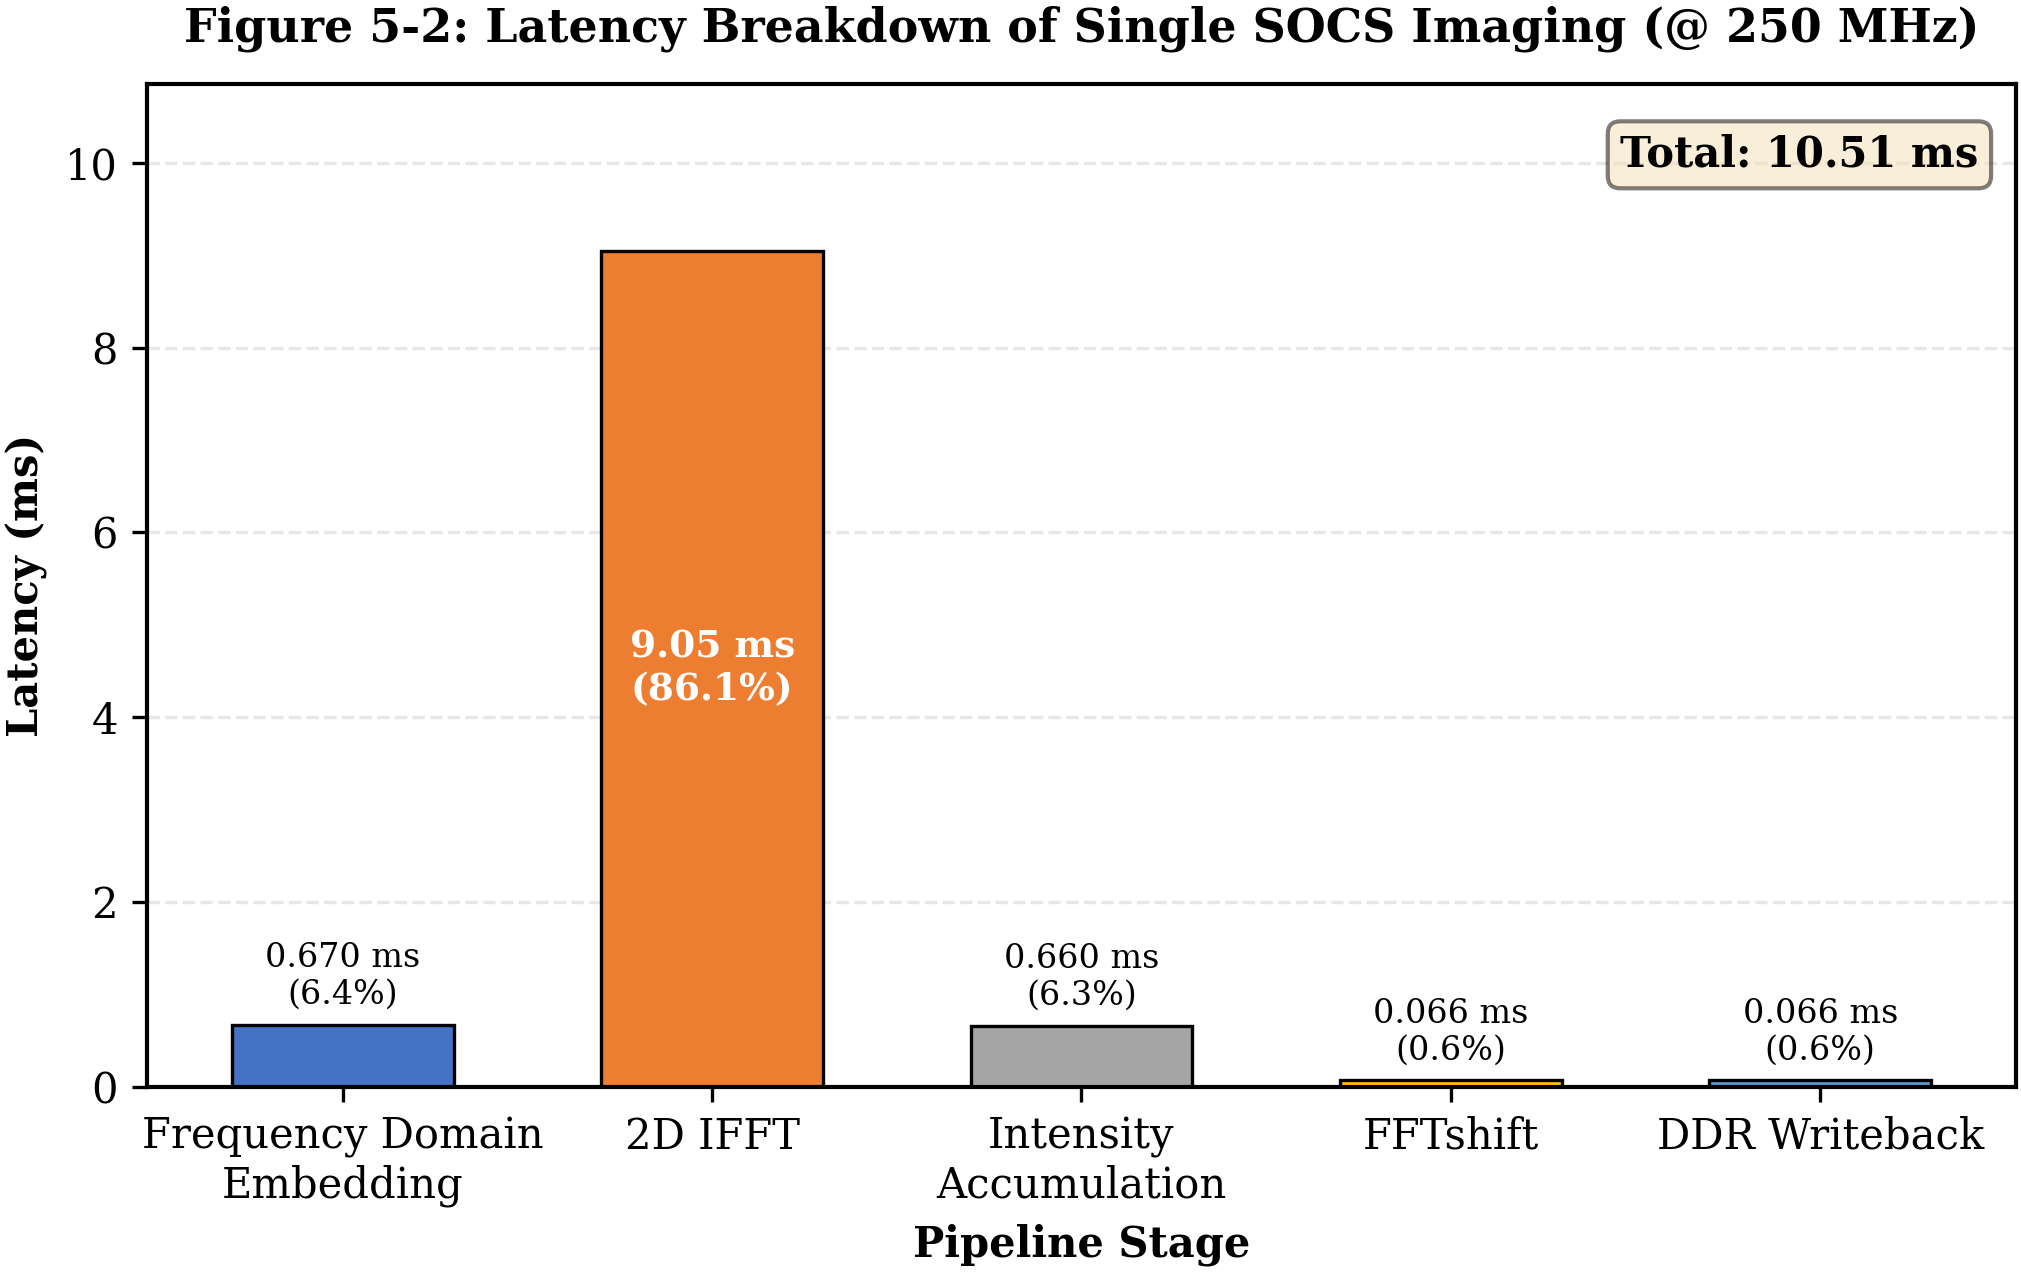
\includegraphics[keepaspectratio,alt={Figure 5 Latency breakdown of the proposed FPGA pipeline}]{../image/论文/ch5_fig2_latency_breakdown.png}}
\caption{Figure 5 Latency breakdown of the proposed FPGA pipeline}
\end{figure}

\textbf{Figure 5} Latency breakdown of the proposed FPGA online
reconstruction kernel.

\subsubsection{3.3.2 CPU-FPGA Speedup}\label{cpu-fpga-speedup}

Table 7 compares only the online reconstruction stage under the same
inputs and 10-kernel SOCS equation. The measured C++ CPU latency is 35.6
ms, whereas the FPGA kernel latency is 10.57 ms, yielding a
\(3.37\times\) speedup and a 70.3\% reduction in per-image latency. The
corresponding throughput increases from 28.09 images/s to 94.6 images/s.
Neither MATLAB execution time nor direct full-TCC imaging time is used
in this comparison, thereby avoiding unfair conclusions caused by
differences in algorithmic scope or implementation accuracy.

\textbf{Table 7} CPU-FPGA performance comparison for the same 10-kernel
SOCS online reconstruction operator

{\def\LTcaptype{none} % do not increment counter
\begin{longtable}[]{@{}
  >{\raggedright\arraybackslash}p{(\linewidth - 8\tabcolsep) * \real{0.220}}
  >{\raggedleft\arraybackslash}p{(\linewidth - 8\tabcolsep) * \real{0.150}}
  >{\raggedleft\arraybackslash}p{(\linewidth - 8\tabcolsep) * \real{0.210}}
  >{\raggedleft\arraybackslash}p{(\linewidth - 8\tabcolsep) * \real{0.210}}
  >{\raggedleft\arraybackslash}p{(\linewidth - 8\tabcolsep) * \real{0.210}}@{}}
\toprule\noalign{}
\begin{minipage}[b]{\linewidth}\raggedright
Platform
\end{minipage} & \begin{minipage}[b]{\linewidth}\raggedleft
Latency
\end{minipage} & \begin{minipage}[b]{\linewidth}\raggedleft
Throughput
\end{minipage} & \begin{minipage}[b]{\linewidth}\raggedleft
Relative speedup
\end{minipage} & \begin{minipage}[b]{\linewidth}\raggedleft
Latency reduction
\end{minipage} \\
\midrule\noalign{}
\endhead
\bottomrule\noalign{}
\endlastfoot
C++ CPU SOCS & 35.6 ms & 28.09 images/s & \(1.00\times\) & - \\
FPGA SOCS kernel & 10.57 ms & 94.6 images/s & \(3.37\times\) & 70.3\% \\
\end{longtable}
}

This speedup arises from the execution architecture rather than a change
in the imaging model. The CPU sequentially performs complex
multiplication, two-dimensional IFFT, and intensity accumulation through
software loops. The FPGA reuses a fixed-size IFFT engine and reduces
control and memory-access overhead through pipelined loops, BRAM
intermediate buffers, and independent AXI-MM channels. For window-level
aerial image computation repeatedly invoked in OPC/SMO/ILT, the 24.99 ms
latency saving per invocation accumulates with the number of calls.

\subsubsection{3.3.3 Energy Consumption per Image and Energy
Efficiency}\label{energy-consumption-per-image-and-energy-efficiency}

To compare the energy consumption per task, the energy required for each
aerial image is calculated as \(E=P\times T\). The current CPU power is
estimated from an approximately 80 W server operating power, while the
FPGA uses an approximately 4 W post-synthesis power estimate for the
online reconstruction kernel. Therefore,

\[
E_{\mathrm{CPU}}=80\times35.6\ \mathrm{ms}=2.848\ \mathrm{J/image},
\qquad\mathrm{(11)}
\]

\[
E_{\mathrm{FPGA}}=4\times10.57\ \mathrm{ms}=0.0423\ \mathrm{J/image}.
\qquad\mathrm{(12)}
\]

As shown in Table 8, under this estimation methodology the FPGA reduces
the energy consumption per image by approximately 98.5\%. Energy
efficiency increases from 0.351 images/J to 23.7 images/J, corresponding
to an approximately \(67.4\times\) improvement in kernel-only energy
efficiency.

\textbf{Table 8} Estimated kernel-only energy-efficiency comparison
between the FPGA and C++ CPU SOCS implementations

{\def\LTcaptype{none} % do not increment counter
\begin{longtable}[]{@{}
  >{\raggedright\arraybackslash}p{(\linewidth - 8\tabcolsep) * \real{0.200}}
  >{\raggedleft\arraybackslash}p{(\linewidth - 8\tabcolsep) * \real{0.145}}
  >{\raggedleft\arraybackslash}p{(\linewidth - 8\tabcolsep) * \real{0.190}}
  >{\raggedleft\arraybackslash}p{(\linewidth - 8\tabcolsep) * \real{0.220}}
  >{\raggedleft\arraybackslash}p{(\linewidth - 8\tabcolsep) * \real{0.245}}@{}}
\toprule\noalign{}
\begin{minipage}[b]{\linewidth}\raggedright
Platform
\end{minipage} & \begin{minipage}[b]{\linewidth}\raggedleft
Latency
\end{minipage} & \begin{minipage}[b]{\linewidth}\raggedleft
Estimated power
\end{minipage} & \begin{minipage}[b]{\linewidth}\raggedleft
Energy per image
\end{minipage} & \begin{minipage}[b]{\linewidth}\raggedleft
Energy efficiency
\end{minipage} \\
\midrule\noalign{}
\endhead
\bottomrule\noalign{}
\endlastfoot
C++ CPU SOCS & 35.6 ms & approximately 80 W & 2.848 J/image & 0.351
images/J \\
FPGA SOCS kernel & 10.57 ms & approximately 4 W & 0.0423 J/image & 23.7
images/J \\
\end{longtable}
}

The \(67.4\times\) value represents only the FPGA kernel-only energy
efficiency derived from the current power estimates; it is not a
full-platform measurement including the Host CPU, PCIe, DDR, and
host-side FI. Before publication, FPGA power should be calibrated using
a Vivado Power Analyzer report with switching-activity information or
on-board sensors, while the CPU baseline power should be measured using
RAPL, BMC, or an external power meter.

\subsubsection{3.3.4 Resource Utilization and System
Boundary}\label{resource-utilization-and-system-boundary}

Table 9 presents the resource utilization of the final design. DSP
utilization is only 2\%, indicating that LUT mapping of FFT
multiplications effectively prevents DSP resources from becoming an
implementation bottleneck. BRAM utilization is 42\%, primarily due to
the two-dimensional IFFT transpose and multi-kernel accumulation
buffers. This resource distribution allows the design to be deployed on
the medium-scale xcku5p device and provides a hardware basis for
low-power operation.

\textbf{Table 9} FPGA resource utilization on the xcku5p

{\def\LTcaptype{none} % do not increment counter
\begin{longtable}[]{@{}lrrr@{}}
\toprule\noalign{}
Resource & Used & Available & Utilization \\
\midrule\noalign{}
\endhead
\bottomrule\noalign{}
\endlastfoot
LUT & 36,931 & 216,960 & 17\% \\
FF & 38,703 & 433,920 & 9\% \\
DSP & 34 & 1,824 & 2\% \\
BRAM\_18K & 399 & 960 & 42\% \\
\end{longtable}
}

\begin{figure}
\centering
\pandocbounded{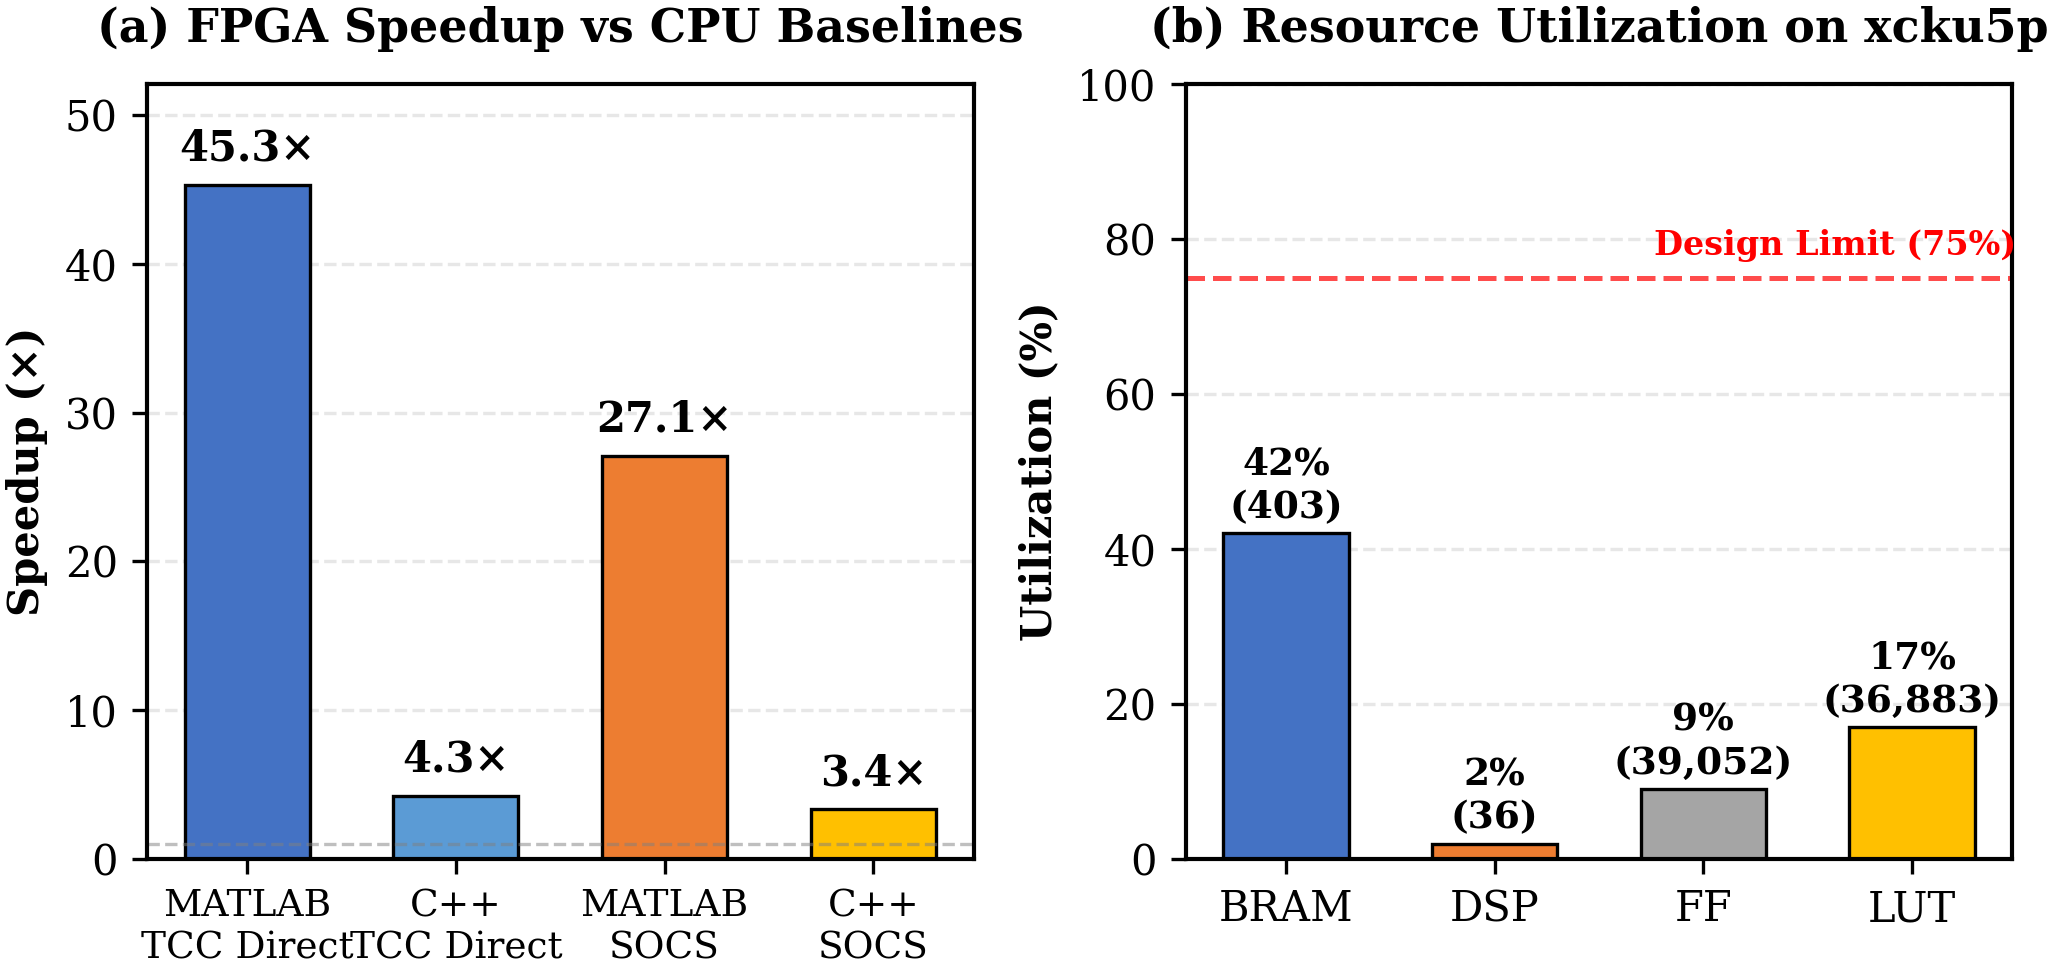
\includegraphics[keepaspectratio,alt={Figure 6 Summary of performance, energy efficiency, and resource utilization}]{../image/论文/ch5_fig3_performance_resource.png}}
\caption{Figure 6 Summary of performance, energy efficiency, and
resource utilization}
\end{figure}

\textbf{Figure 6} Summary of the performance, estimated kernel-only
energy efficiency, and resource utilization of the proposed FPGA/HLS
architecture.

PCIe XDMA on-board data writes, AXI-Lite control, result read-back, and
Host FI have also been validated. This single-window system path
includes host system calls, DMA, polling, and post-processing, and
therefore uses a timing scope different from the computation-only
results in Table 7. It is not included in the calculation of the
\(3.37\times\) kernel speedup or the estimated \(67.4\times\)
kernel-only energy-efficiency improvement. GPUs are better suited to
computational lithography tasks that prioritize maximum throughput over
large batches. Rather than making a quantitative comparison using
unrelated public data, this work positions the proposed architecture as
an online reconstruction kernel targeting low power and deterministic
latency.

Taken together, the experiments under the fixed configuration establish
a complete chain of evidence. The MATLAB comparison defines the
model-accuracy bound of the 10-kernel SOCS approximation, on-board
validation demonstrates that the FPGA hardware implementation error is
substantially below this bound, and the same-operator CPU comparison
confirms that the FPGA reduces online latency and estimated energy
consumption per image while preserving the imaging result. These
conclusions apply only to the TCC-SOCS online reconstruction kernel and
should not be extrapolated to the complete OPC/SMO toolchain or the
energy efficiency of the full Host-FPGA system.

\section{4. Conclusions}\label{conclusions}

This paper proposes a low-latency and energy-efficient FPGA architecture
for TCC-SOCS aerial image reconstruction. Its central principle is to
retain optical-system-dependent TCC construction and SOCS eigenkernel
extraction on the CPU while mapping the frequently executed online
reconstruction stage in OPC/SMO workflows to a dedicated FPGA datapath.
PCIe XDMA integrates input-data writes, AXI-Lite control, result
read-back, and host-side Fourier interpolation into a complete execution
path. Through this partitioning, the complex optical model is compressed
into reusable eigenkernels and weights, while the FPGA performs only
regular operations, including frequency-domain embedding,
two-dimensional IFFT, weighted accumulation, FFTshift, and result
write-back. The online computational hotspot of TCC-SOCS is thereby
transformed into a pipelineable and deployable hardware task.

Experiments under the fixed configuration validate this partitioning in
terms of accuracy, latency, and energy consumption. The RMSE of the
10-kernel SOCS result relative to the full MATLAB TCC result is
\(5.472\times10^{-3}\), whereas the on-board FPGA output and Host FI
result have RMSE values of \(2.93\times10^{-8}\) and
\(2.95\times10^{-8}\), respectively, relative to the SOCS software
Golden result under the same configuration. The hardware implementation
error is therefore substantially smaller than the model truncation
error. Through block-floating-point FFT scaling, LUT-mapped FFT
multiplication, multi-port AXI-MM access, and BRAM buffering, the design
achieves a 10-kernel online reconstruction kernel latency of 10.57 ms at
250 MHz on the xcku5p FPGA. Compared with the C++ CPU SOCS baseline
implementing the same operator, latency is reduced by 70.3\%,
corresponding to a \(3.37\times\) speedup. Based on the current FPGA
kernel and CPU power estimates of approximately 4 W and 80 W,
respectively, the energy consumption per image decreases from 2.848 J to
0.0423 J, corresponding to an estimated \(67.4\times\) improvement in
kernel-only energy efficiency. The final architecture utilizes 17\% of
the LUTs, 9\% of the FFs, 2\% of the DSPs, and 42\% of the BRAM. For the
repeated evaluation of numerous small-window aerial images in
computational lithography, these results indicate that FPGAs are well
suited to low-power TCC-SOCS online reconstruction with deterministic
latency.

The current validation targets the TCC-SOCS online reconstruction kernel
and its PCIe on-board profile path; it does not claim end-to-end
acceleration of a complete OPC/SMO toolchain. Future deployments may
increase inter-kernel SOCS parallelism on devices with larger BRAM
capacity, support adaptive FFT-grid sizes, integrate Fourier
interpolation and post-processing into the FPGA pipeline, optimize
batched PCIe transfers and interrupt control, and extend the approach to
dipole, quasar, high-NA EUV, and larger industrial mask patterns. The
proposed architecture can thereby evolve from validation of an online
reconstruction kernel into an energy-efficient CPU-FPGA collaborative
acceleration system for practical computational lithography workflows.

\section{References}\label{references}

\begin{enumerate}
\def\labelenumi{\arabic{enumi}.}
\tightlist
\item
  Granik Y. Fast pixel-based mask optimization for inverse
  lithography{[}J{]}. Journal of Micro/Nanolithography, MEMS and MOEMS,
  2006, 5(4): 043002-043002-13.
\item
  Cobb N B, Zakhor A, Miloslavsky E A. Mathematical and CAD framework
  for proximity correction{[}C{]}//Optical Microlithography IX. SPIE,
  1996, 2726: 208-222.
\item
  Jia N, Lam E Y. Pixelated source mask optimization for process
  robustness in optical lithography{[}J{]}. Optics express, 2011,
  19(20): 19384-19398.
\item
  Li Z, Dong L, Ma X, et al.~Fast source mask co-optimization method for
  high-NA EUV lithography{[}J{]}. Opto-Electronic Advances, 2025, 7(4):
  230235-1-230235-11.
\item
  Shen Y, Wong N, Lam E Y. Level-set-based inverse lithography for
  photomask synthesis{[}J{]}. Optics Express, 2009, 17(26): 23690-23701.
\item
  Abrams D S, Pang L. Fast inverse lithography
  technology{[}C{]}//Optical Microlithography XIX. SPIE, 2006, 6154:
  534-542.
\item
  Pang L, Liu Y, Abrams D. Inverse lithography technology (ILT): What is
  the impact to the photomask industry?{[}C{]}//Photomask and
  Next-Generation Lithography Mask Technology XIII. SPIE, 2006, 6283:
  233-243.
\item
  Gao J R, Xu X, Yu B, et al.~MOSAIC: Mask optimizing solution with
  process window aware inverse correction{[}C{]}//Proceedings of the
  51st Annual Design Automation Conference. 2014: 1-6.
\item
  Kim B G, Suh S S, Kim B S, et al.~Trade-off between inverse
  lithography mask complexity and lithographic
  performance{[}C{]}//Photomask and Next-Generation Lithography Mask
  Technology XVI. SPIE, 2009, 7379: 458-468.
\item
  Pang L, Liu Y, Abrams D. Inverse lithography technology (ILT): a
  natural solution for model-based SRAF at 45-nm and
  32-nm{[}C{]}//Photomask and Next-Generation Lithography Mask
  Technology XIV. SPIE, 2007, 6607: 888-897.
\item
  Hung C Y, Zhang B, Guo E, et al.~Pushing the lithography limit:
  Applying inverse lithography technology (ILT) at the 65nm
  generation{[}C{]}//Optical Microlithography XIX. SPIE, 2006, 6154:
  562-571.
\item
  Ma X, Arce G. Binary mask optimization for inverse lithography with
  partially coherent illumination{[}J{]}. Journal of the optical society
  of America A, 2008, 25(12): 2960-2970.
\item
  Maa X, Arceb G R. PSM design for inverse lithography with partially
  coherent illumination{[}J{]}. Optics express, 2008, 16(24):
  20126-20141.
\item
  Yeung M S, Lee D, Lee R S, et al.~Extension of the Hopkins theory of
  partially coherent imaging to include thin-film interference
  effects{[}C{]}//Optical/Laser Microlithography. SPIE, 1993, 1927:
  452-463.
\item
  Adam K, Granik Y, Torres A, et al.~Improved modeling performance with
  an adapted vectorial formulation of the Hopkins imaging
  equation{[}C{]}//Optical Microlithography XVI. SPIE, 2003, 5040:
  78-91.
\item
  Gong P, Liu S, Lv W, et al.~Fast aerial image simulations for
  partially coherent systems by transmission cross coefficient
  decomposition with analytical kernels{[}J{]}. Journal of Vacuum
  Science \& Technology B, 2012, 30(6).
\item
  Köhle R. Fast TCC algorithm for the model building of high NA
  lithography simulation{[}C{]}//Optical Microlithography XVIII. SPIE,
  2005, 5754: 918-929.
\item
  Wu X, Liu S, Liu W, et al.~Comparison of three TCC calculation
  algorithms for partially coherent imaging simulation{[}C{]}//Sixth
  International Symposium on Precision Engineering Measurements and
  Instrumentation. SPIE, 2010, 7544: 241-250.
\item
  Yu P, Pan D Z. ELIAS: an accurate and extensible lithography aerial
  image simulator with improved numerical algorithms{[}J{]}. IEEE
  transactions on semiconductor manufacturing, 2009, 22(2): 276-289.
\item
  Yu P, Qiu W, Pan D Z. Fast lithography image simulation by exploiting
  symmetries in lithography systems{[}J{]}. IEEE transactions on
  semiconductor manufacturing, 2008, 21(4): 638-645.
\item
  Bernard D A, Li J, Rey J C, et al.~Efficient computational techniques
  for aerial imaging simulation{[}C{]}//Optical Microlithography IX.
  SPIE, 1996, 2726: 273-287.
\item
  Rodrigues R, Sreedhar A, Kundu S. Optical lithography simulation using
  wavelet transform{[}C{]}//2009 IEEE International Conference on
  Computer Design. IEEE, 2009: 427-432.
\item
  Zheng X, Ma X, Zhao Q, et al.~Model-informed deep learning for
  computational lithography with partially coherent illumination{[}J{]}.
  Optics Express, 2020, 28(26): 39475-39491.
\item
  Torunoglu I, Karakas A, Elsen E, et al.~OPC on a single desktop: a
  GPU-based OPC and verification tool for fabs and
  designers{[}C{]}//Design for Manufacturability through Design-Process
  Integration IV. SPIE, 2010, 7641.
\item
  Yu Z, Chen G, Ma Y, et al.~A GPU-Enabled Level-Set Method for Mask
  Optimization{[}J{]}. IEEE Transactions on Computer-Aided Design of
  Integrated Circuits and Systems, 2023, 42(2): 594-605.
\item
  Yang H, Li S, Deng Z, et al.~GAN-OPC: Mask Optimization With
  Lithography-Guided Generative Adversarial Nets{[}J{]}. IEEE
  Transactions on Computer-Aided Design of Integrated Circuits and
  Systems, 2020, 39(10): 2822-2834.
\item
  Ye W, Alawieh M B, Lin Y, et al.~LithoGAN{[}C{]}//Proceedings of the
  56th Annual Design Automation Conference 2019. ACM, 2019: 1-6.
\item
  Jiang B, Liu L, Ma Y, et al.~Neural-ILT 2.0: Migrating ILT to
  Domain-Specific and Multitask-Enabled Neural Network{[}J{]}. IEEE
  Transactions on Computer-Aided Design of Integrated Circuits and
  Systems, 2022, 41(8): 2671-2684.
\item
  Chen G, Chen W, Sun Q, et al.~DAMO: Deep Agile Mask Optimization for
  Full-Chip Scale{[}J{]}. IEEE Transactions on Computer-Aided Design of
  Integrated Circuits and Systems, 2022, 41(9): 3118-3131.
\item
  Yang H, Li Z, Sastry K, et al.~Generic lithography modeling with
  dual-band optics-inspired neural networks{[}C{]}//Proceedings of the
  59th ACM/IEEE Design Automation Conference. ACM, 2022: 973-978.
\item
  Cong J, Zou Y. FPGA-Based Hardware Acceleration of Lithographic Aerial
  Image Simulation{[}J{]}. ACM Transactions on Reconfigurable Technology
  and Systems, 2009, 2(3): 1-29.
\item
  Cong J, Zou Y. Lithographic aerial image simulation with FPGA-based
  hardwareacceleration{[}C{]}//Proceedings of the 16th international
  ACM/SIGDA symposium on Field programmable gate arrays. ACM, 2008:
  67-76.
\item
  Akin B, Milder P A, Franchetti F, et al.~Memory Bandwidth Efficient
  Two-Dimensional Fast Fourier Transform Algorithm and Implementation
  for Large Problem Sizes{[}C{]}//2012 IEEE 20th International Symposium
  on Field-Programmable Custom Computing Machines. IEEE, 2012.
\item
  Akin B, Franchetti F, Hoe J C. Understanding the design space of
  DRAM-optimized hardware FFT accelerators{[}C{]}//2014 IEEE 25th
  International Conference on Application-Specific Systems,
  Architectures and Processors. IEEE, 2014: 248-255.
\item
  Chen R, Prasanna V K. Energy optimizations for FPGA-based 2-D FFT
  architecture{[}C{]}//2014 IEEE High Performance Extreme Computing
  Conference (HPEC). IEEE, 2014: 1-6.
\item
  Chen R, Le H, Prasanna V K. Energy efficient parameterized FFT
  architecture{[}C{]}//2013 23rd International Conference on Field
  programmable Logic and Applications. IEEE, 2013: 1-7.
\item
  Seonil Choi, Govindu G, Ju-Wook Jang, et al.~Energy-efficient and
  parameterized designs for fast Fourier transform on FPGAs{[}C{]}//2003
  IEEE International Conference on Acoustics, Speech, and Signal
  Processing, 2003. Proceedings. (ICASSP '03). IEEE, 2003, 2: II-521-4.
\item
  Tang S N, Liao C H, Chang T Y. An Area- and Energy-Efficient Multimode
  FFT Processor for WPAN/WLAN/WMAN Systems{[}J{]}. IEEE Journal of
  Solid-State Circuits, 2012, 47(6): 1419-1435.
\end{enumerate}

\end{document}
